\chapter{Methodology}

% Include dynamically generated statistics
% Automatically generated data quality statistics
% Generated: 2025-09-28 18:18:32

% Overall statistics
\renewcommand{\TheTotalNumberCustomers}{41,285}
\renewcommand{\TheInitialYear}{2019}
\renewcommand{\TheFinalYear}{2024}
\renewcommand{\TheTotalCustomerYears}{212,924}

% Customer data availability
\renewcommand{\CustomerNumberOneYear}{25,347}
\renewcommand{\CustomerPctOneYear}{61.4}
\renewcommand{\CustomerNumberTwoPlusYear}{14,995}
\renewcommand{\CustomerPctTwoPlusYear}{36.3}
\renewcommand{\CustomerNumberNoData}{15,938}
\renewcommand{\CustomerPctNoData}{38.6}

% Exclusion statistics
\renewcommand{\ExclusionMidYearQSICount}{957}
\renewcommand{\ExclusionMidYearQSIPct}{0.5}
\renewcommand{\ExclusionLateEntryCount}{43,102}
\renewcommand{\ExclusionLateEntryPct}{20.2}
\renewcommand{\ExclusionEarlyExitCount}{14,873}
\renewcommand{\ExclusionEarlyExitPct}{7.0}
\renewcommand{\ExclusionNoCostsCount}{109}
\renewcommand{\ExclusionNoCostsPct}{0.1}
\renewcommand{\ExclusionInsufficientServiceCount}{81,901}
\renewcommand{\ExclusionInsufficientServicePct}{38.5}
\renewcommand{\ExclusionNoQSICount}{128,791}
\renewcommand{\ExclusionNoQSIPct}{60.5}

% Cost statistics
\renewcommand{\AvgAnnualCost}{\$33,987}
\renewcommand{\MedianAnnualCost}{\$15,454}
\renewcommand{\StdevAnnualCost}{\$40,545}

% Trajectory analysis
\renewcommand{\CustomersWithTrajectory}{14,995}
\renewcommand{\PctWithTrajectory}{36.3}
\renewcommand{\CustomersWithGaps}{177}
\renewcommand{\PctWithGaps}{0.4}

% Outlier statistics
\renewcommand{\OutlierLowerFence}{\$-153,231}
\renewcommand{\OutlierUpperFence}{\$261,983}
\renewcommand{\OutliersBelow}{0}
\renewcommand{\OutliersAbove}{111}
\renewcommand{\OutlierRate}{0.23}


\section{Overview}

This chapter presents the comprehensive methodology for calibrating and evaluating ten alternative models for the Florida iBudget algorithm. The framework addresses significant data quality challenges, implements sophisticated outlier detection strategies, and ensures reproducibility through a unified pipeline architecture. The approach balances statistical rigor with practical constraints imposed by incomplete longitudinal data and irregular service utilization patterns.

% ⚠ ======================================== ⚠ 
% ⚠  DO *NOT* EDIT data_quality_commands.tex ⚠ 
% ⚠  DO *NOT* EDIT data_quality_analysis.tex ⚠ 
% ⚠ ======================================== ⚠ 
% These files are produced by executing the program Outliers.py
% Any change in those files will be lost with every execution of the analysis pipeline 
% Automatically generated data quality statistics
% Generated: 2025-09-28 18:18:32

% Overall statistics
\renewcommand{\TheTotalNumberCustomers}{41,285}
\renewcommand{\TheInitialYear}{2019}
\renewcommand{\TheFinalYear}{2024}
\renewcommand{\TheTotalCustomerYears}{212,924}

% Customer data availability
\renewcommand{\CustomerNumberOneYear}{25,347}
\renewcommand{\CustomerPctOneYear}{61.4}
\renewcommand{\CustomerNumberTwoPlusYear}{14,995}
\renewcommand{\CustomerPctTwoPlusYear}{36.3}
\renewcommand{\CustomerNumberNoData}{15,938}
\renewcommand{\CustomerPctNoData}{38.6}

% Exclusion statistics
\renewcommand{\ExclusionMidYearQSICount}{957}
\renewcommand{\ExclusionMidYearQSIPct}{0.5}
\renewcommand{\ExclusionLateEntryCount}{43,102}
\renewcommand{\ExclusionLateEntryPct}{20.2}
\renewcommand{\ExclusionEarlyExitCount}{14,873}
\renewcommand{\ExclusionEarlyExitPct}{7.0}
\renewcommand{\ExclusionNoCostsCount}{109}
\renewcommand{\ExclusionNoCostsPct}{0.1}
\renewcommand{\ExclusionInsufficientServiceCount}{81,901}
\renewcommand{\ExclusionInsufficientServicePct}{38.5}
\renewcommand{\ExclusionNoQSICount}{128,791}
\renewcommand{\ExclusionNoQSIPct}{60.5}

% Cost statistics
\renewcommand{\AvgAnnualCost}{\$33,987}
\renewcommand{\MedianAnnualCost}{\$15,454}
\renewcommand{\StdevAnnualCost}{\$40,545}

% Trajectory analysis
\renewcommand{\CustomersWithTrajectory}{14,995}
\renewcommand{\PctWithTrajectory}{36.3}
\renewcommand{\CustomersWithGaps}{177}
\renewcommand{\PctWithGaps}{0.4}

% Outlier statistics
\renewcommand{\OutlierLowerFence}{\$-153,231}
\renewcommand{\OutlierUpperFence}{\$261,983}
\renewcommand{\OutliersBelow}{0}
\renewcommand{\OutliersAbove}{111}
\renewcommand{\OutlierRate}{0.23}

\section{Data Quality and Outlier Analysis}

\subsection{Overview}

This section presents a comprehensive analysis of data quality and outlier identification for the iBudget model calibration. The analysis examines customer-year records to identify data quality issues and determine the usable dataset for model development.

\subsection{Data Availability Assessment}

The initial data quality analysis examined \TheTotalNumberCustomers{} unique customers in the Agency for Persons with Disabilities (APD) database, spanning fiscal years \TheInitialYear{} through \TheFinalYear{}. Each fiscal year runs from September 1 through August 31, creating potential complications when Questionnaire for Situational Information (QSI) assessments occur mid-year.

The outlier analysis revealed substantial data quality challenges:
\begin{itemize}
    \item \textbf{\CustomerNumberOneYear{} customers (\CustomerPctOneYear\%)} have at least one fiscal year of usable data
    \item \textbf{\CustomerNumberTwoPlusYear{} customers (\CustomerPctTwoPlusYear\%)} have two or more years suitable for trajectory modeling
    \item \textbf{\CustomerNumberNoData{} customers (\CustomerPctNoData\%)} have no usable data after applying quality criteria
\end{itemize}

\subsection{Customer Coverage Analysis}

\begin{figure}[h]
    \centering
    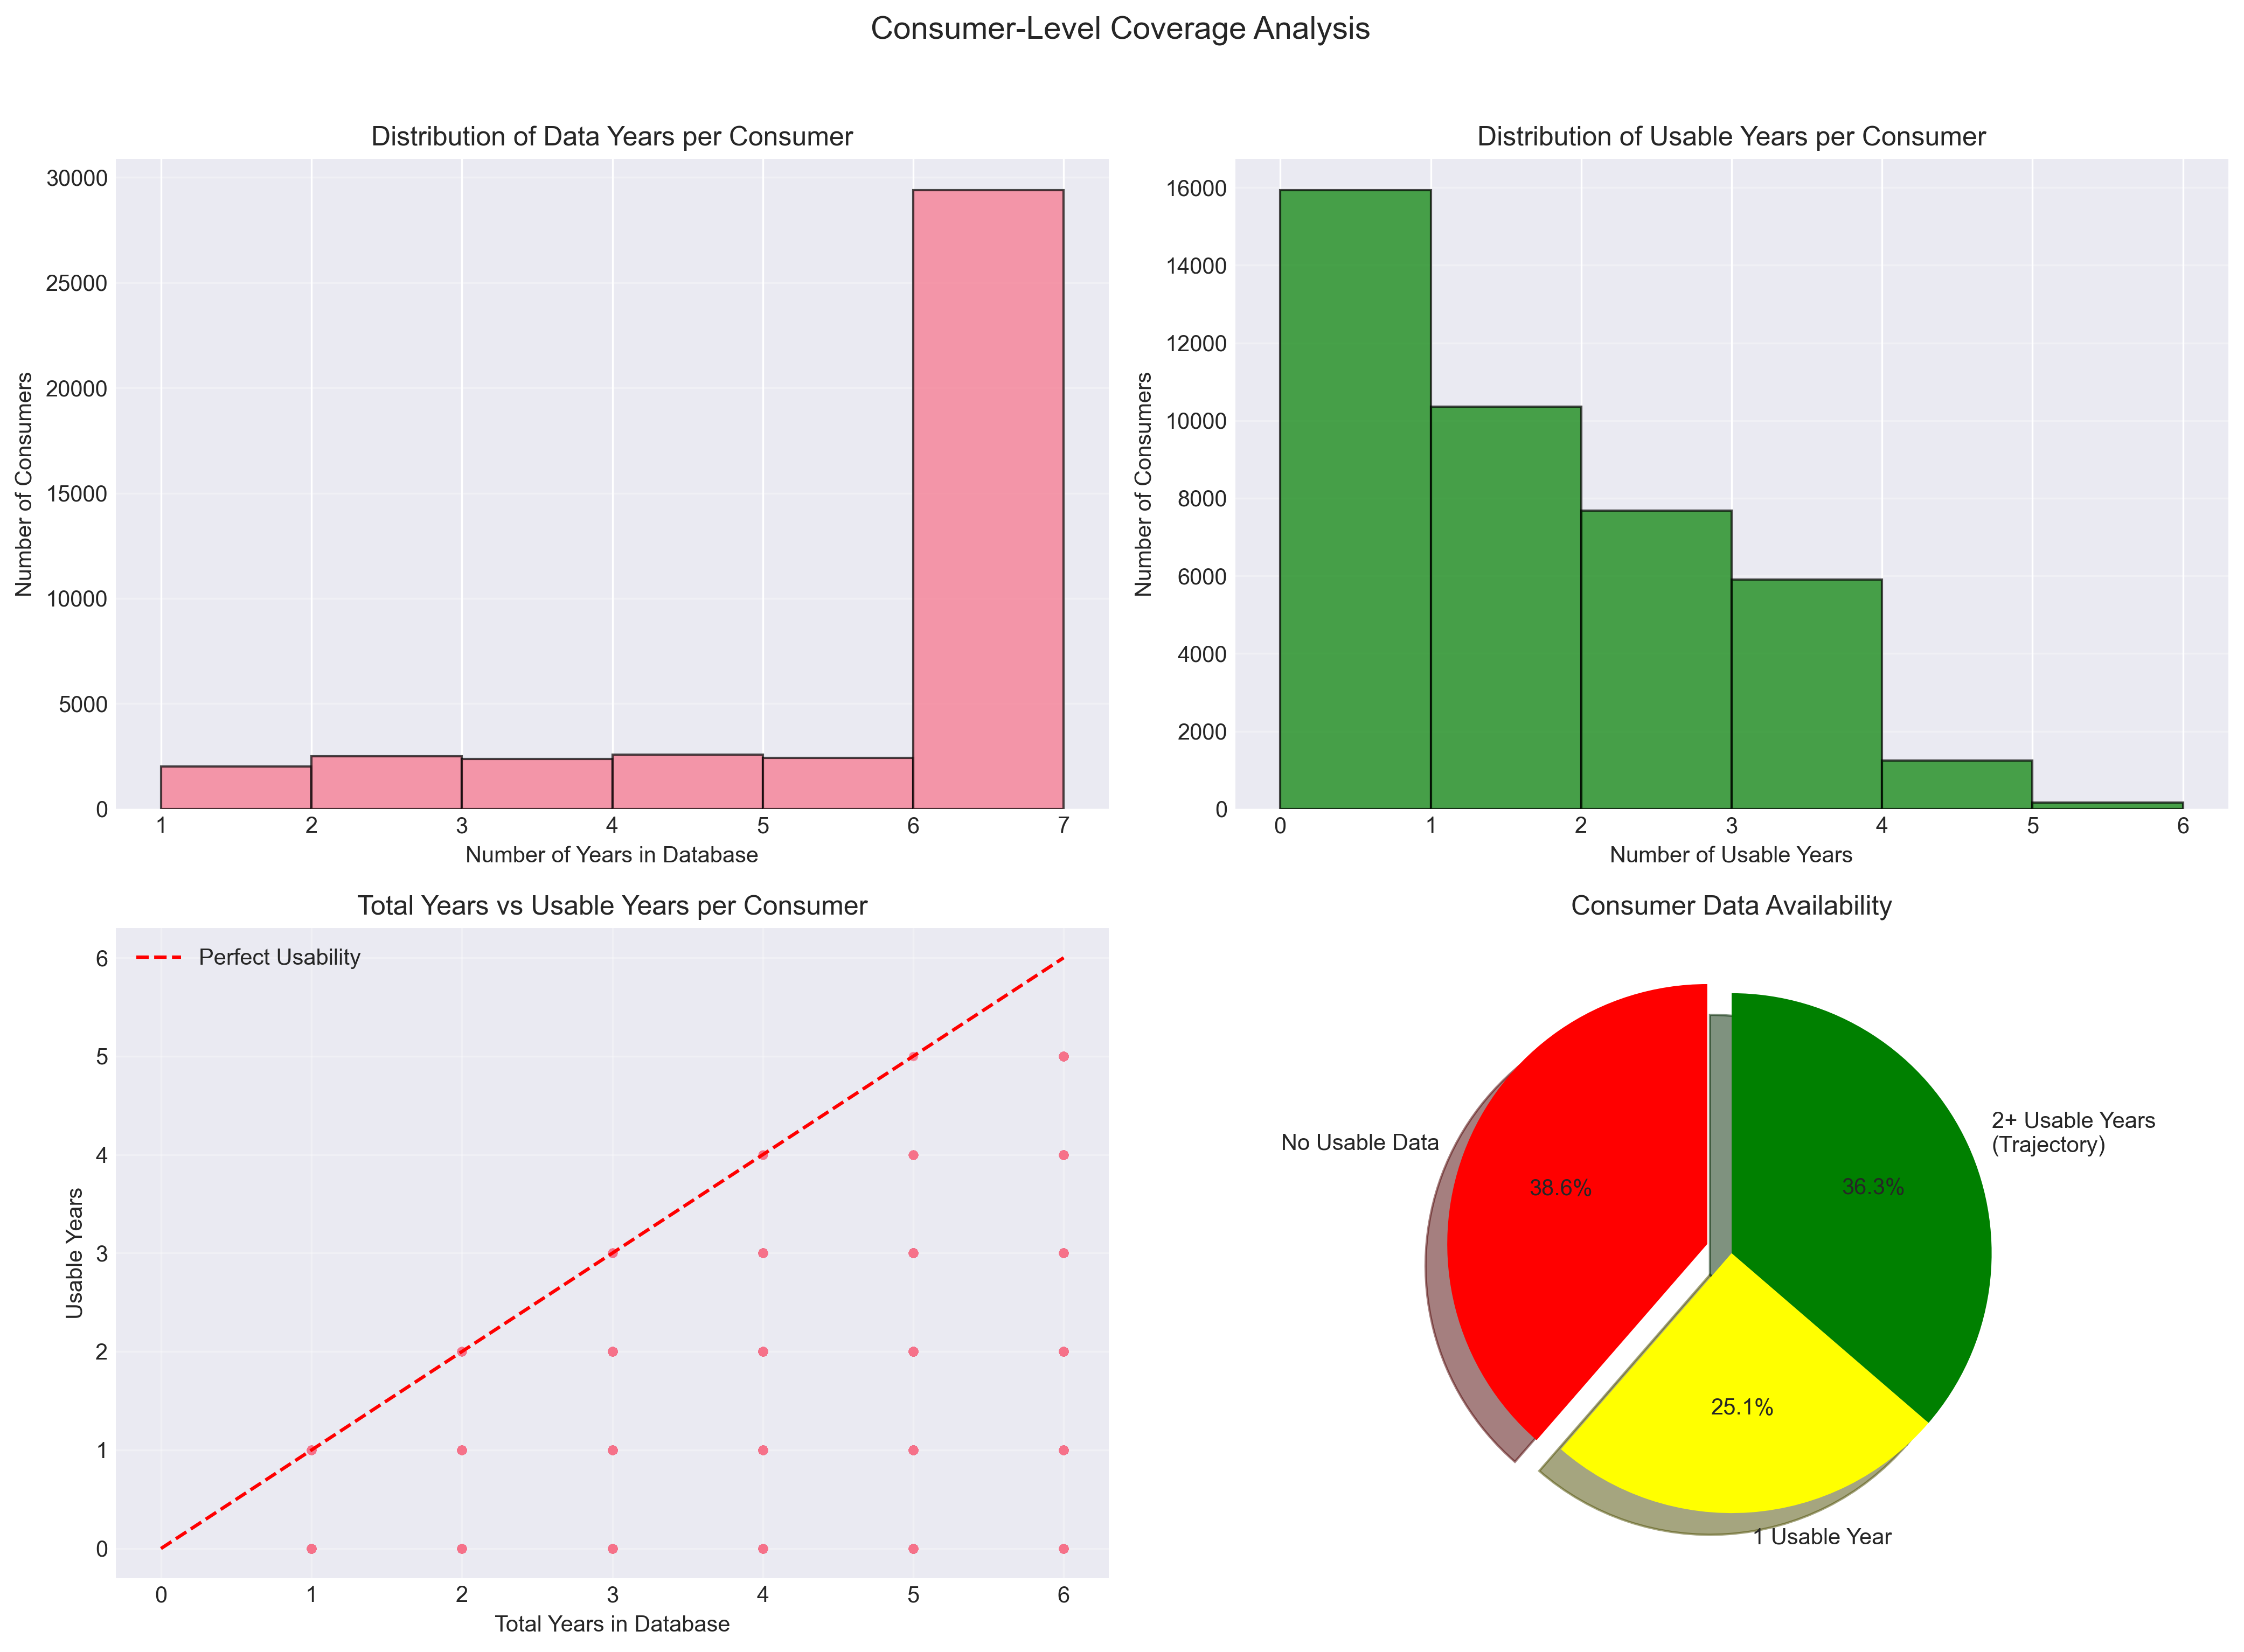
\includegraphics[width=\textwidth]{figures/consumer_coverage.png}
    \caption{Customer-level data coverage analysis}
    \label{fig:customer_coverage}
\end{figure}

Figure~\ref{fig:customer_coverage} presents four panels analyzing customer data availability:
\begin{itemize}
    \item \textbf{Top-left panel}: Distribution of total years each customer appears in the database, showing most customers have either 1-2 years or the full span of data
    \item \textbf{Top-right panel}: Distribution of usable years after applying quality criteria, revealing significant data loss for many customers
    \item \textbf{Bottom-left panel}: Scatter plot comparing total versus usable years, with the red diagonal line representing perfect data usability; points below the line indicate data quality issues
    \item \textbf{Bottom-right panel}: Pie chart showing the critical breakdown---only \CustomerPctTwoPlusYear\% of customers have sufficient data for trajectory modeling
\end{itemize}

\subsection{Data Exclusion Analysis}

Customer-year records are evaluated for several quality issues that would compromise model calibration:

\begin{table}[h]
\centering
\caption{Exclusion Reasons and Impact}
\begin{tabular}{lrr}
\toprule
\textbf{Exclusion Reason} & \textbf{Count} & \textbf{Percentage} \\
\midrule
Mid-Year QSI Change & \ExclusionMidYearQSICount & \ExclusionMidYearQSIPct\% \\
Late Entry (>30 days) & \ExclusionLateEntryCount & \ExclusionLateEntryPct\% \\
Early Exit (>30 days) & \ExclusionEarlyExitCount & \ExclusionEarlyExitPct\% \\
No Costs Recorded & \ExclusionNoCostsCount & \ExclusionNoCostsPct\% \\
Insufficient Service Days & \ExclusionInsufficientServiceCount & \ExclusionInsufficientServicePct\% \\
No QSI Assessment & \ExclusionNoQSICount & \ExclusionNoQSIPct\% \\
\bottomrule
\end{tabular}
\end{table}

\begin{figure}[h]
    \centering
    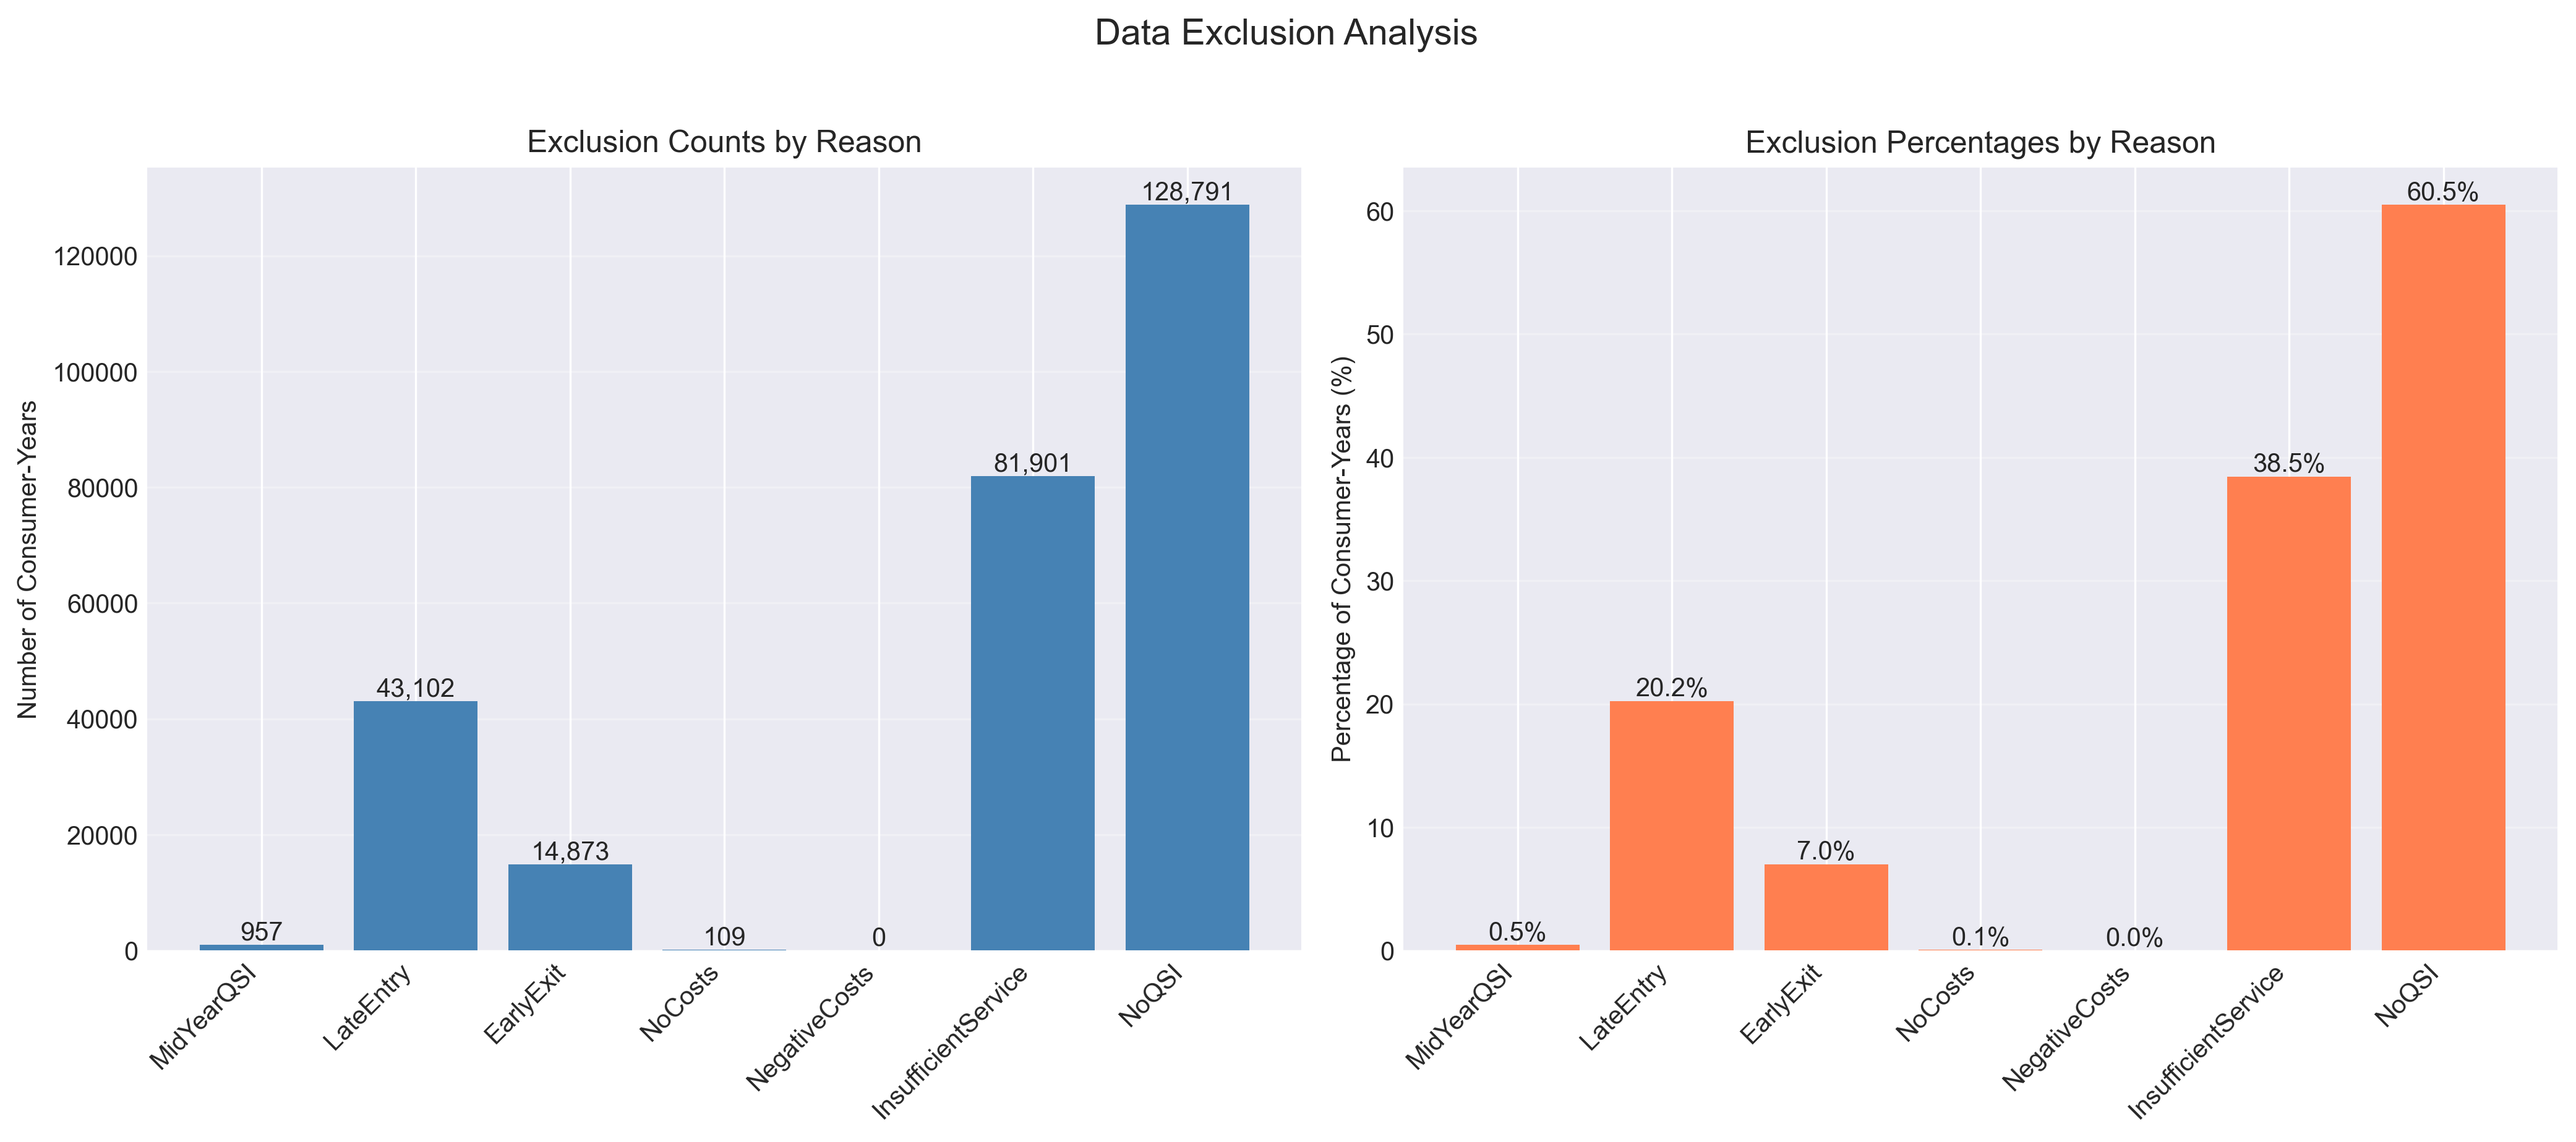
\includegraphics[width=\textwidth]{figures/exclusion_reasons.png}
    \caption{Distribution of exclusion reasons}
    \label{fig:exclusion_reasons}
\end{figure}

Figure~\ref{fig:exclusion_reasons} visualizes the exclusion analysis:
\begin{itemize}
    \item \textbf{Left panel}: Absolute counts of customer-years excluded for each reason, showing the scale of data loss
    \item \textbf{Right panel}: Percentage breakdown highlighting that mid-year QSI changes and incomplete fiscal years are the primary exclusion drivers
\end{itemize}

\subsection{Cost Distribution Analysis}

\begin{figure}[h]
    \centering
    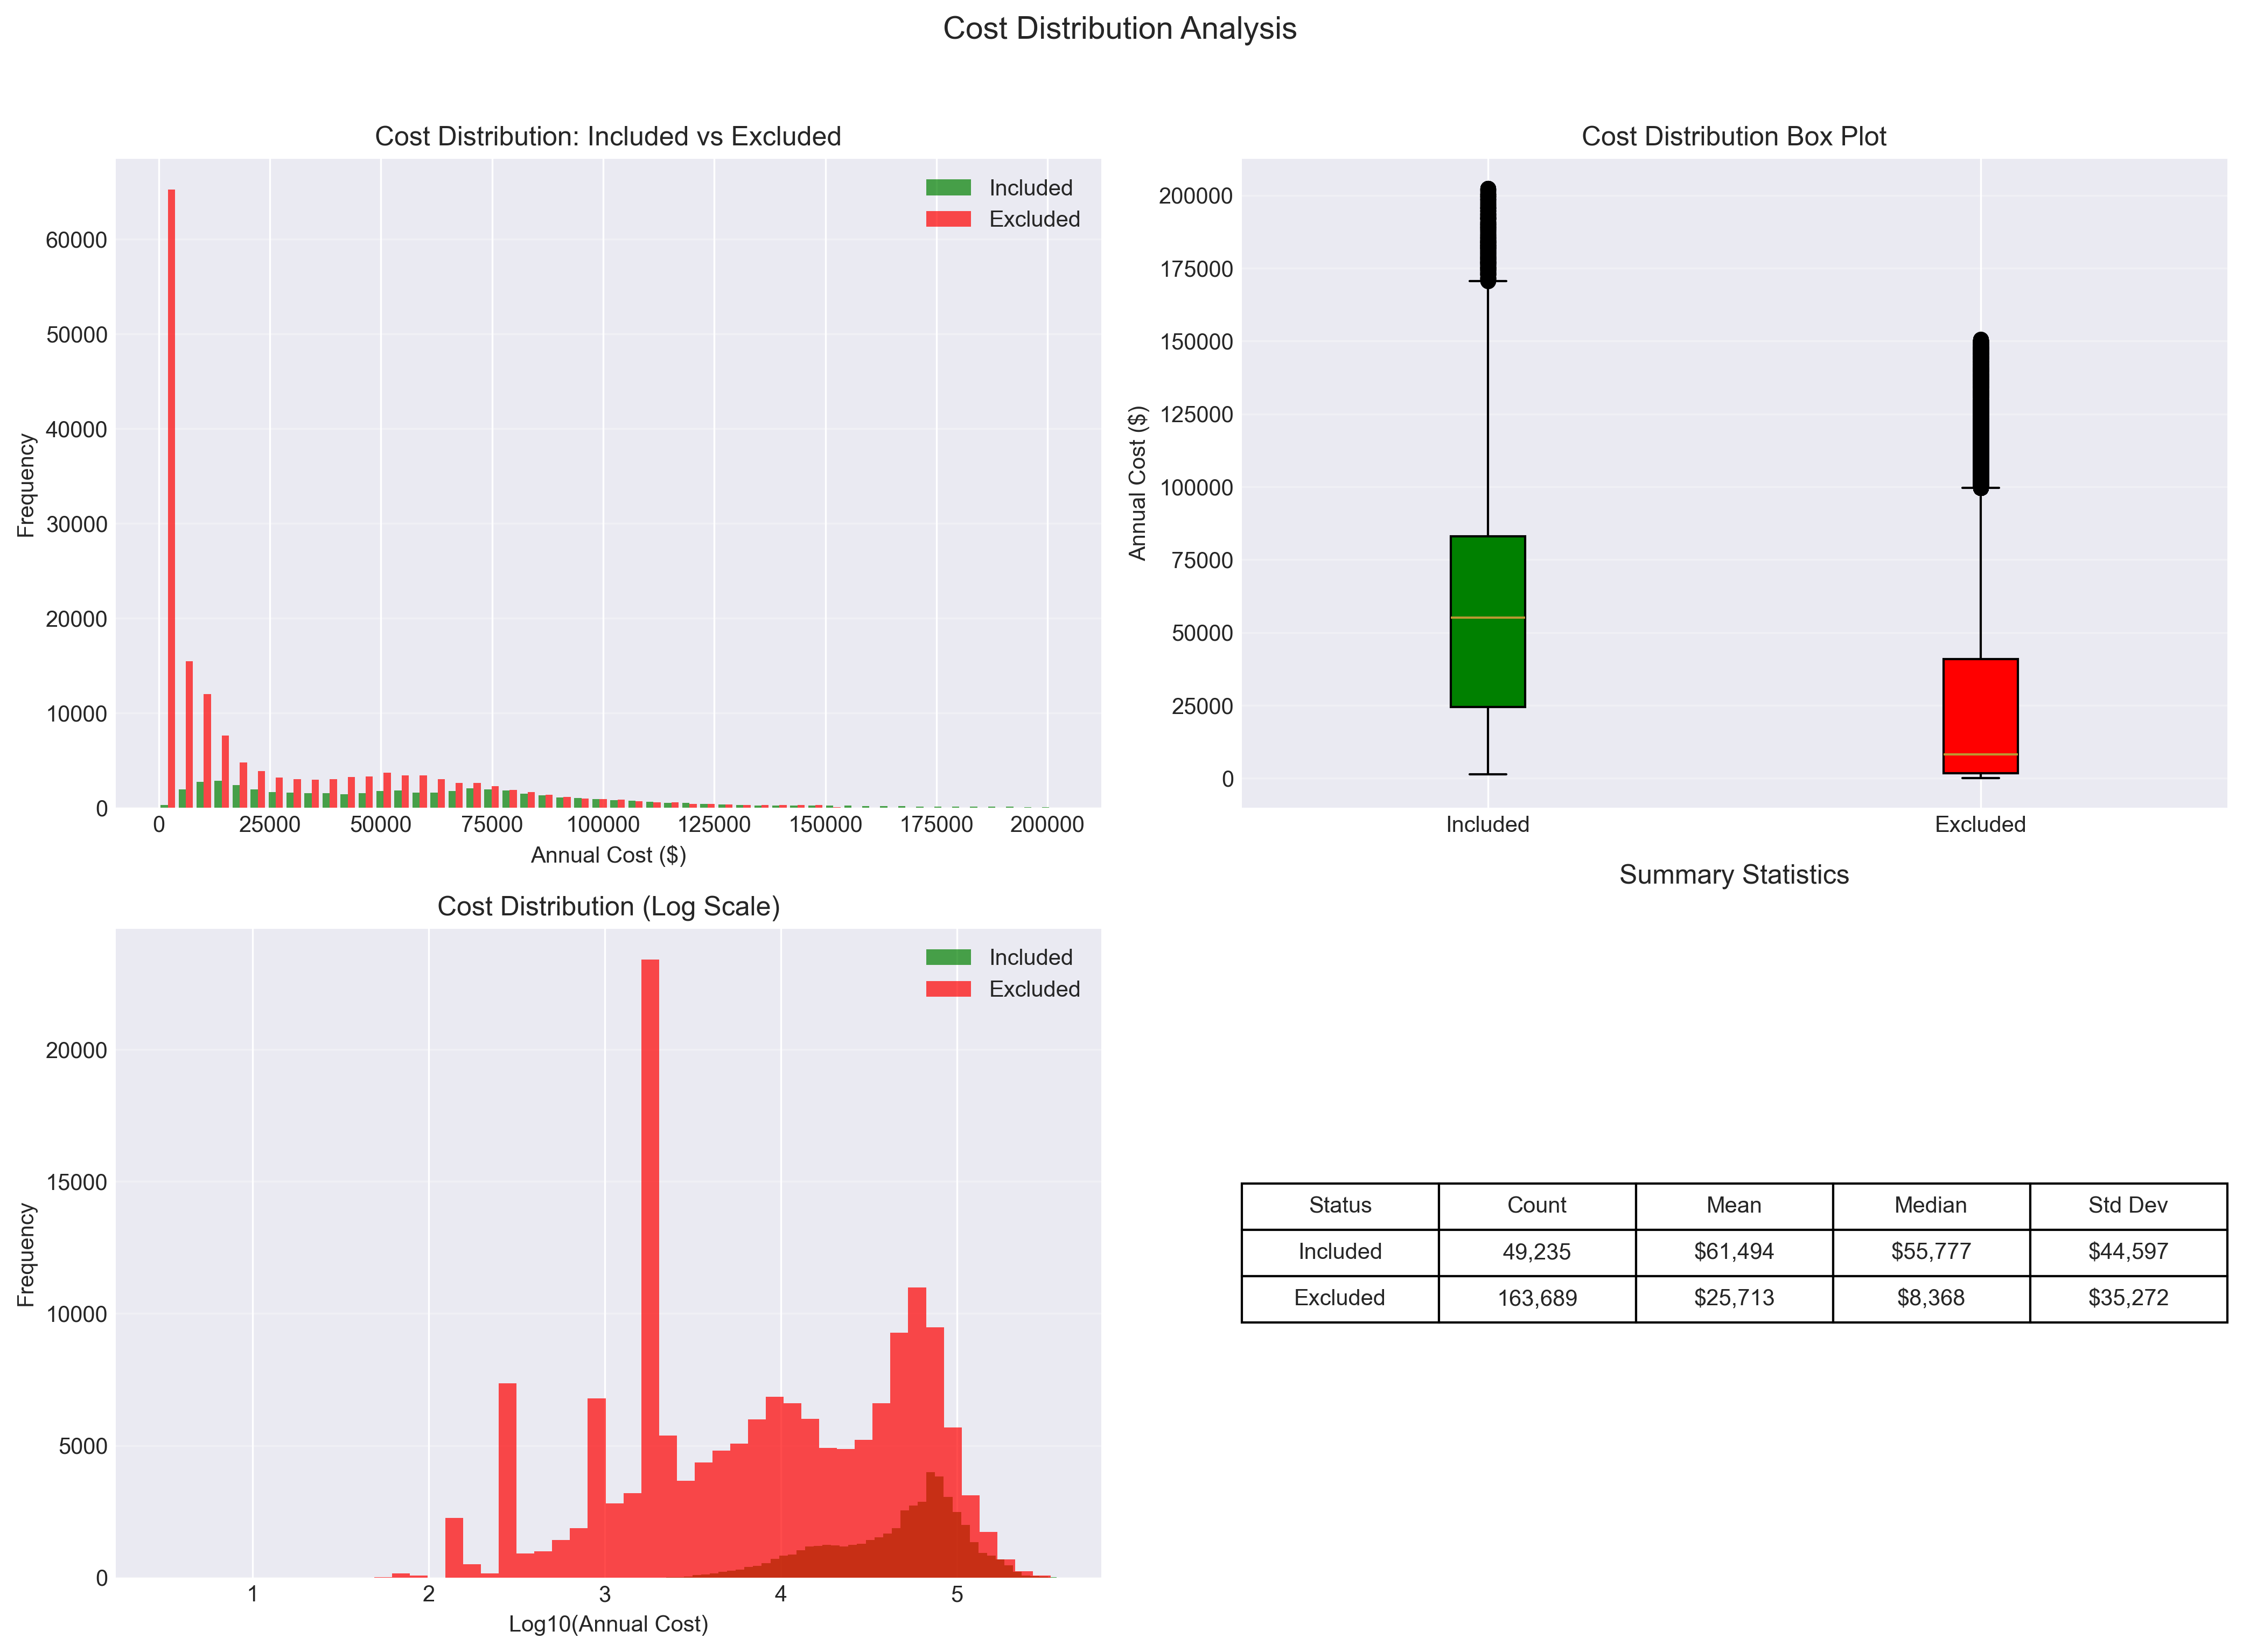
\includegraphics[width=\textwidth]{figures/cost_distributions.png}
    \caption{Comparison of cost distributions between included and excluded customer-years}
    \label{fig:cost_distributions}
\end{figure}

Figure~\ref{fig:cost_distributions} compares cost patterns between included and excluded data:
\begin{itemize}
    \item \textbf{Top-left}: Histogram overlay showing excluded records tend toward lower costs
    \item \textbf{Top-right}: Box plots revealing excluded records have wider variance and more outliers
    \item \textbf{Bottom-left}: Log-scale distribution highlighting the heavy tail in both populations
    \item \textbf{Bottom-right}: Summary statistics confirming systematically different cost profiles
\end{itemize}

\subsection{Temporal Trends}

\begin{figure}[h]
    \centering
    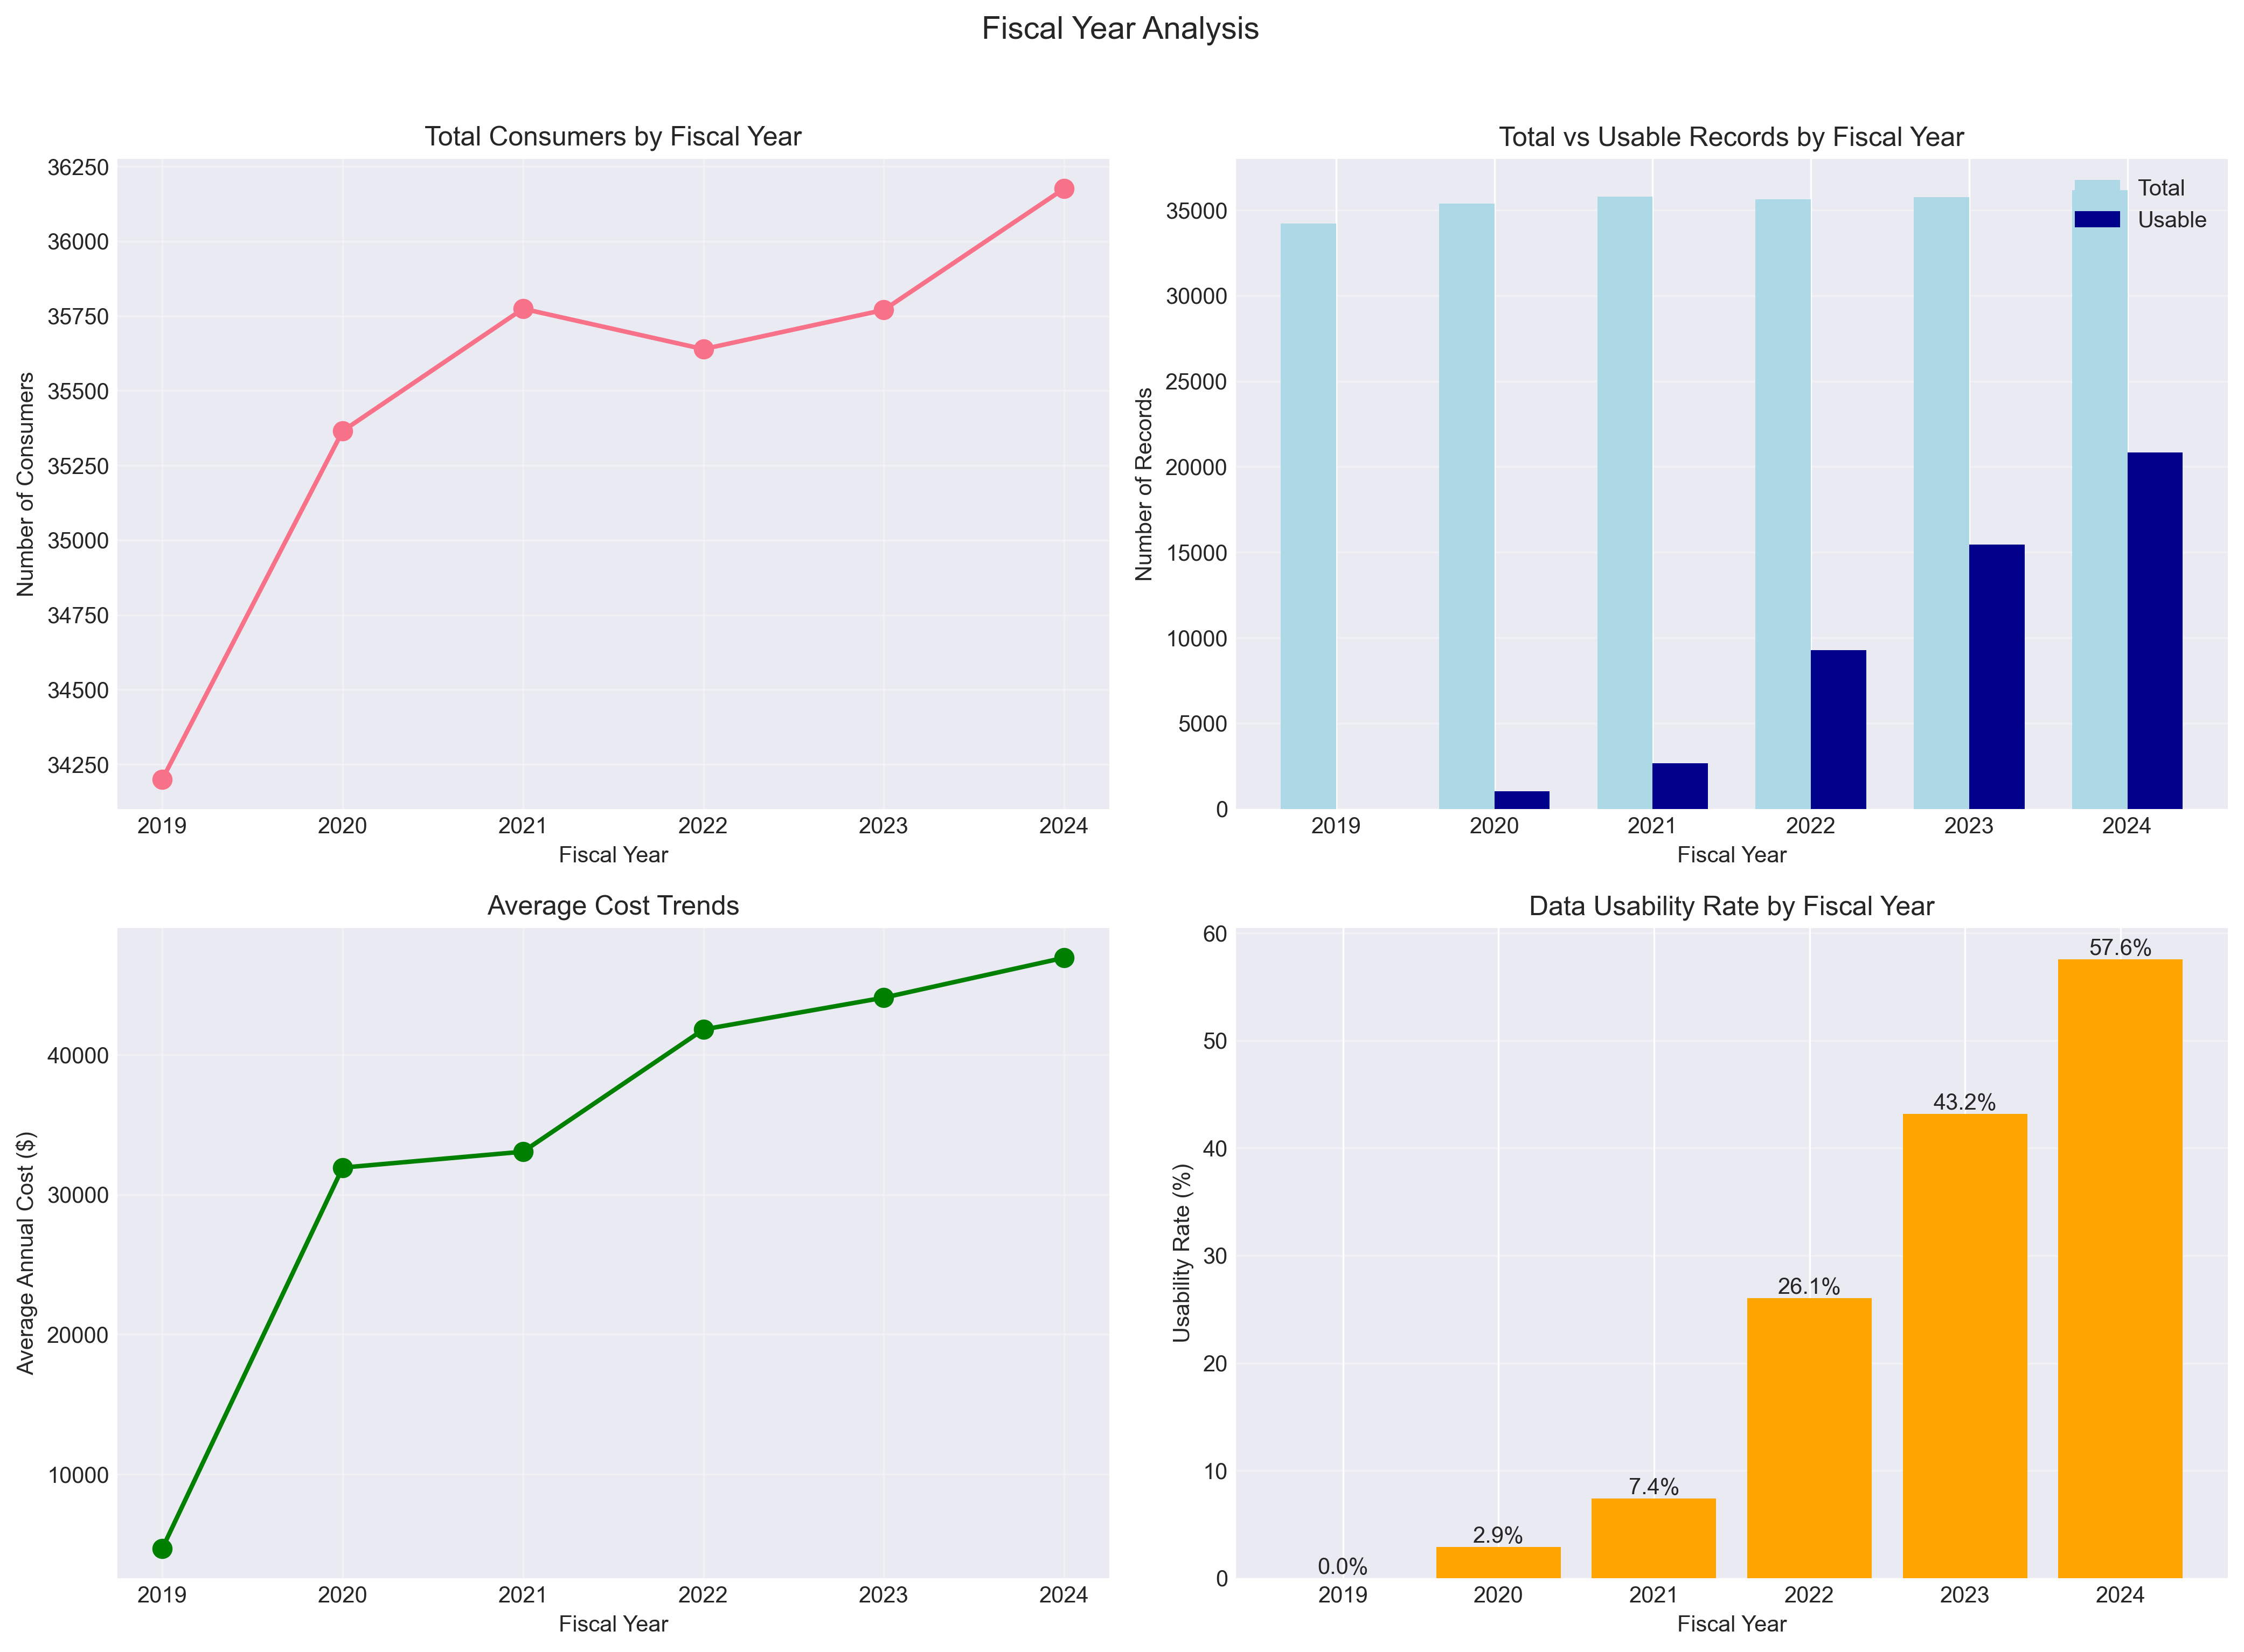
\includegraphics[width=\textwidth]{figures/fiscal_year_trends.png}
    \caption{Trends across fiscal years}
    \label{fig:fiscal_year_trends}
\end{figure}

Figure~\ref{fig:fiscal_year_trends} examines patterns over time:
\begin{itemize}
    \item \textbf{Top-left}: Customer counts by fiscal year show program growth
    \item \textbf{Top-right}: Comparison of total versus usable records reveals consistent data quality challenges
    \item \textbf{Bottom-left}: Average costs trending upward, reflecting inflation and service expansion
    \item \textbf{Bottom-right}: Data usability rates remain relatively stable across years
\end{itemize}

\subsection{Cost Outlier Analysis}

Using the Tukey method with a 3$\times$IQR threshold for extreme outliers:
\begin{itemize}
    \item Lower fence: \OutlierLowerFence
    \item Upper fence: \OutlierUpperFence
    \item Outliers below lower fence: \OutliersBelow
    \item Outliers above upper fence: \OutliersAbove
    \item Total outlier rate: \OutlierRate\%
\end{itemize}

\begin{figure}[h]
    \centering
    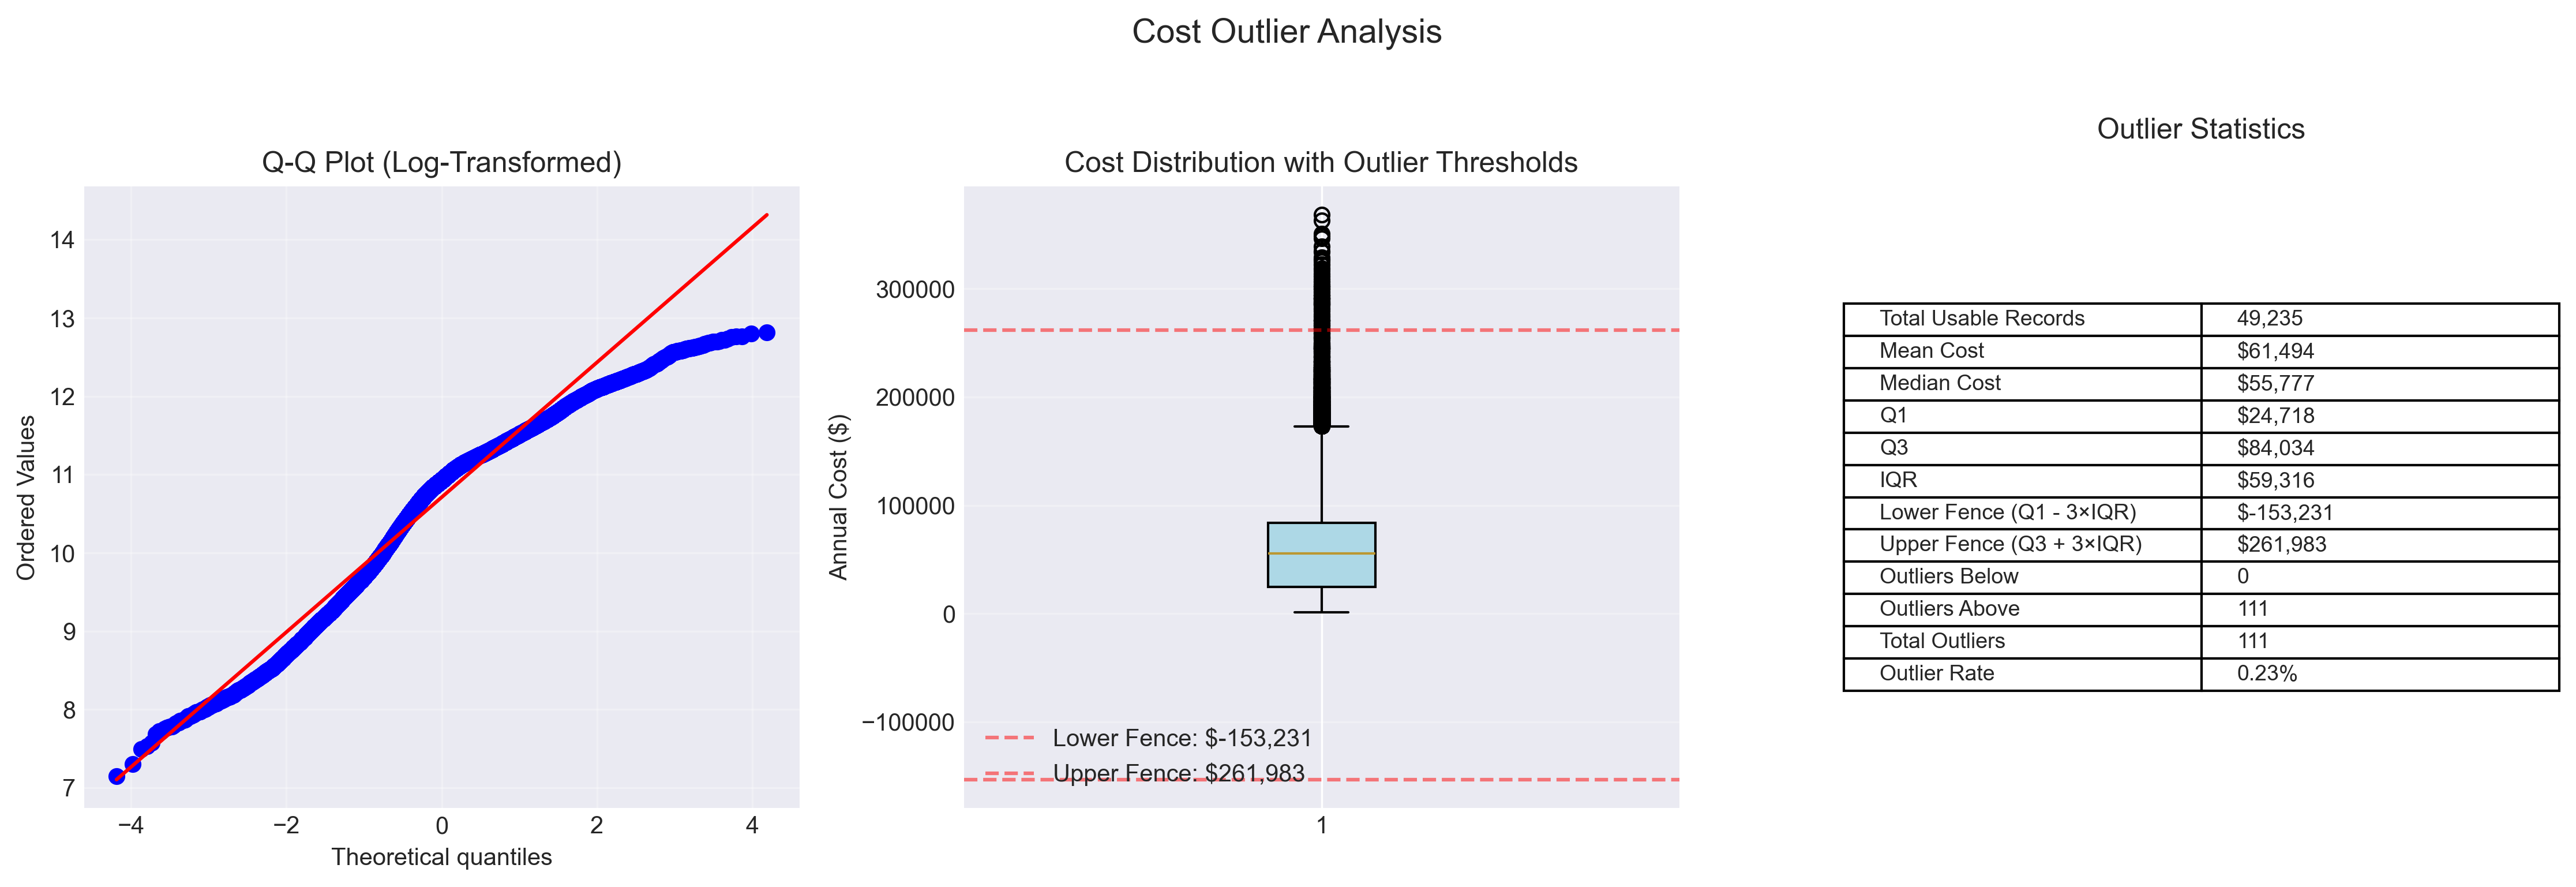
\includegraphics[width=\textwidth]{figures/cost_outliers.png}
    \caption{Cost outlier analysis}
    \label{fig:cost_outliers}
\end{figure}

Figure~\ref{fig:cost_outliers} provides outlier diagnostics:
\begin{itemize}
    \item \textbf{Left panel}: Q-Q plot of log-transformed costs shows approximate normality with heavy tails
    \item \textbf{Center panel}: Box plot with outlier thresholds (red dashed lines) identifies extreme values
    \item \textbf{Right panel}: Statistical summary quantifying outlier prevalence
\end{itemize}

\subsection{Exclusion Overlap Analysis}

\begin{figure}[h]
    \centering
    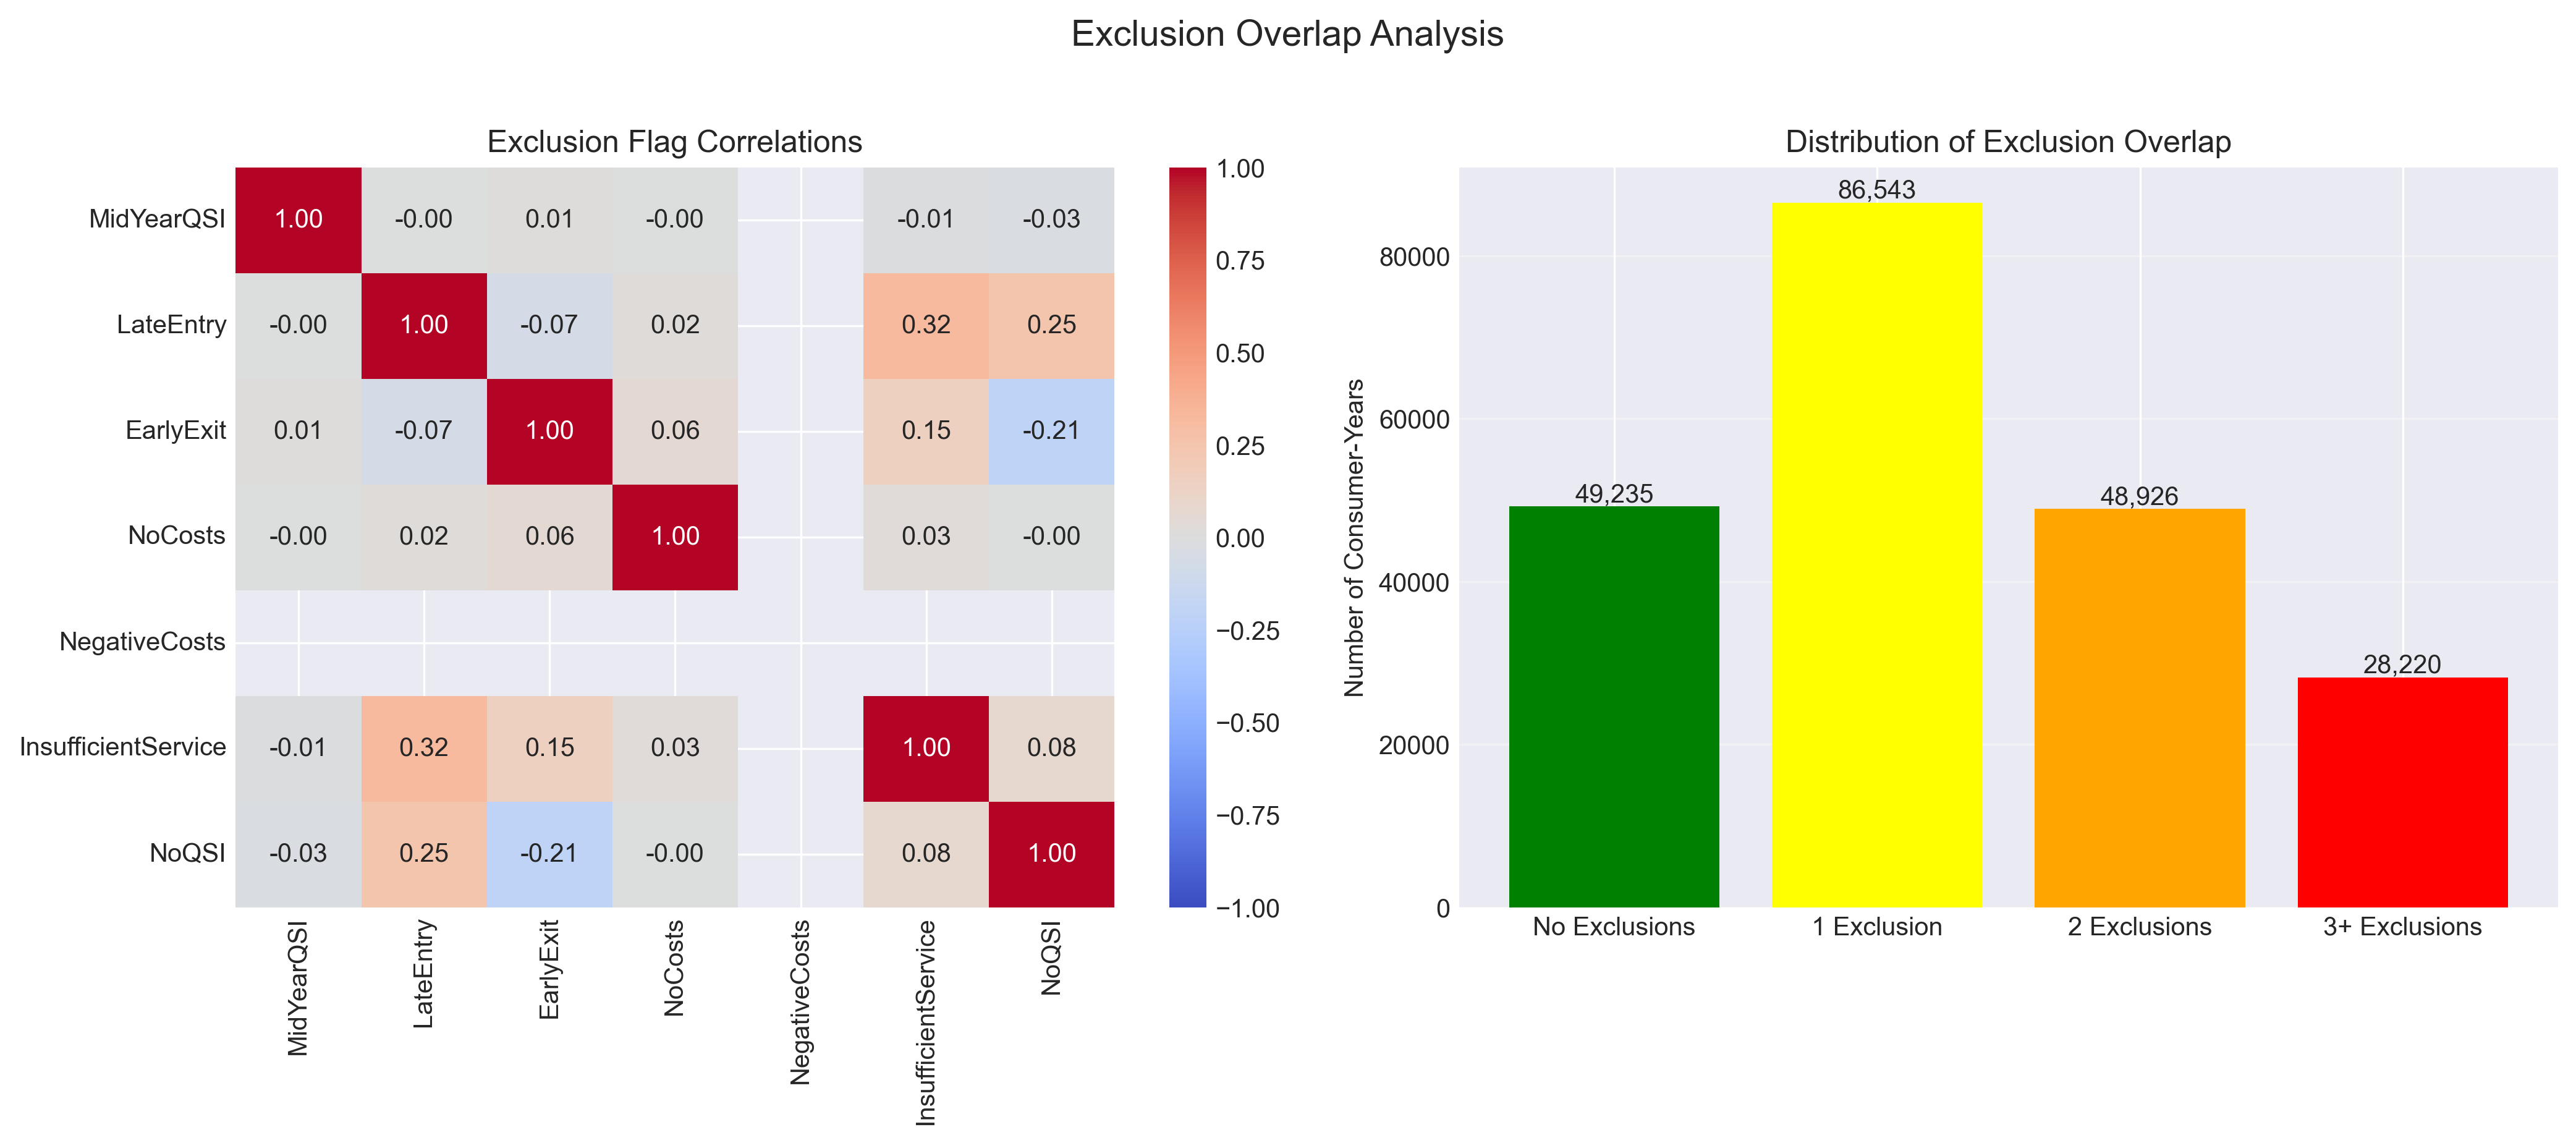
\includegraphics[width=\textwidth]{figures/exclusion_overlap.png}
    \caption{Analysis of exclusion flag correlations and overlap}
    \label{fig:exclusion_overlap}
\end{figure}

Figure~\ref{fig:exclusion_overlap} examines relationships between exclusion criteria:
\begin{itemize}
    \item \textbf{Left panel}: Correlation heatmap reveals which exclusion reasons tend to co-occur (red indicates positive correlation)
    \item \textbf{Right panel}: Bar chart showing most excluded records have multiple issues, justifying the conservative approach
\end{itemize}

\subsection{Trajectory Analysis Feasibility}

For the proposed individual trajectory modeling:
\begin{itemize}
    \item \textbf{\CustomersWithTrajectory{} customers (\PctWithTrajectory\%)} have sufficient data for individual trajectory calculation
    \item \textbf{\CustomersWithGaps{} customers (\PctWithGaps\%)} have gaps in their yearly data
    \item Customers without multi-year data will require group-based trajectory imputation
\end{itemize}

\subsection{Recommendations}

Based on this analysis:

\begin{enumerate}
    \item \textbf{Data Sufficiency}: With \CustomerPctOneYear\% of customers having usable data and \CustomerPctTwoPlusYear\% having multi-year data, the dataset supports model calibration but requires careful handling of limited trajectory coverage.
    
    \item \textbf{Trajectory Modeling}: The proposed trajectory approach is feasible for approximately \PctWithTrajectory\% of customers. The remaining customers will require cluster-based imputation.
    
    \item \textbf{Exclusion Strategy}: The conservative approach excluding customer-years with mid-year QSI changes affects \ExclusionMidYearQSIPct\% of records but ensures clean QSI-to-cost mapping.
    
    \item \textbf{Model Robustness}: Models should be tested for sensitivity to the exclusion criteria and validated on both included and excluded populations where feasible.
\end{enumerate}

% ⚠ ======================================== ⚠ 

\section{Data Quality and Exclusion Strategy}

\subsection{Data Availability Assessment}

The initial data quality analysis examined \TheTotalNumberCustomers{} unique customers in the Agency for Persons with Disabilities (APD) database, spanning fiscal years \TheInitialYear{} through \TheFinalYear{}. Each fiscal year runs from September 1 through August 31, creating potential complications when Questionnaire for Situational Information (QSI) assessments occur mid-year.

The outlier analysis revealed substantial data quality challenges:
\begin{itemize}
    \item \textbf{\CustomerNumberOneYear{} customers (\CustomerPctOneYear\%)} have at least one fiscal year of usable data
    \item \textbf{\CustomerNumberTwoPlusYear{} customers (\CustomerPctTwoPlusYear\%)} have two or more years suitable for trajectory modeling
    \item \textbf{\CustomerNumberNoData{} customers (\CustomerPctNoData\%)} have no usable data after applying quality criteria
\end{itemize}

\subsection{Exclusion Criteria}

Customer-fiscal year records are excluded from calibration if they exhibit any of the following characteristics:

\begin{enumerate}
    \item \textbf{Mid-year QSI changes}: Multiple QSI assessments within a single fiscal year create ambiguity in attributing costs to specific QSI scores
    \item \textbf{Late entry}: Customers entering the system more than 30 days after fiscal year start
    \item \textbf{Early exit}: Customers leaving the system more than 30 days before fiscal year end
    \item \textbf{Zero or negative costs}: Records with \$0 or negative total paid amounts
    \item \textbf{Insufficient service days}: Fewer than 30 service days within the fiscal year
    \item \textbf{Missing QSI assessment}: No QSI assessment linked to the fiscal year
\end{enumerate}

This conservative approach prioritizes data quality over quantity, ensuring that model calibration uses only complete, unambiguous customer-year records.

% ⚠ ===================================== ⚠ 
% ⚠  DO *NOT* EDIT proration_commands.tex ⚠ 
% ⚠  DO *NOT* EDIT proration_analysis.tex ⚠ 
% ⚠ ===================================== ⚠ 
% These file are produced by executing the program ProrationAnalysis.py
% Any change in those files will be lost with every execution of the analysis pipeline 
% Proration Analysis Statistics
% Generated: 2025-09-28 18:55:04

% Coverage statistics
\renewcommand{\ProrationFullYearPct}{70.3}
\renewcommand{\ProrationHighCoveragePct}{78.2}
\renewcommand{\ProrationMedianRFull}{754.80}
\renewcommand{\ProrationMedianRLow}{1.96}

% Customer counts
\renewcommand{\ProrationTotalCustomerYears}{212,924}
\renewcommand{\ProrationFullYearCount}{149,702}
\renewcommand{\ProrationHighCoverageCount}{166,577}

\subsection{Proration Analysis and Decision}

Given the substantial data loss from excluding mid-year QSI changes, we investigated whether costs could be prorated for partial-year records. The analysis examined monthly cost distributions for all customers, calculating two metrics:

\begin{align}
q &= \frac{\text{months with services}}{12} \\
r &= \sum_{i=1}^{12} \frac{(m_i - \bar{m})^2}{\bar{m}}
\end{align}

where $m_i$ represents monthly expenses and $\bar{m}$ is the average monthly expense for that customer-year.

\begin{figure}[h]
    \centering
    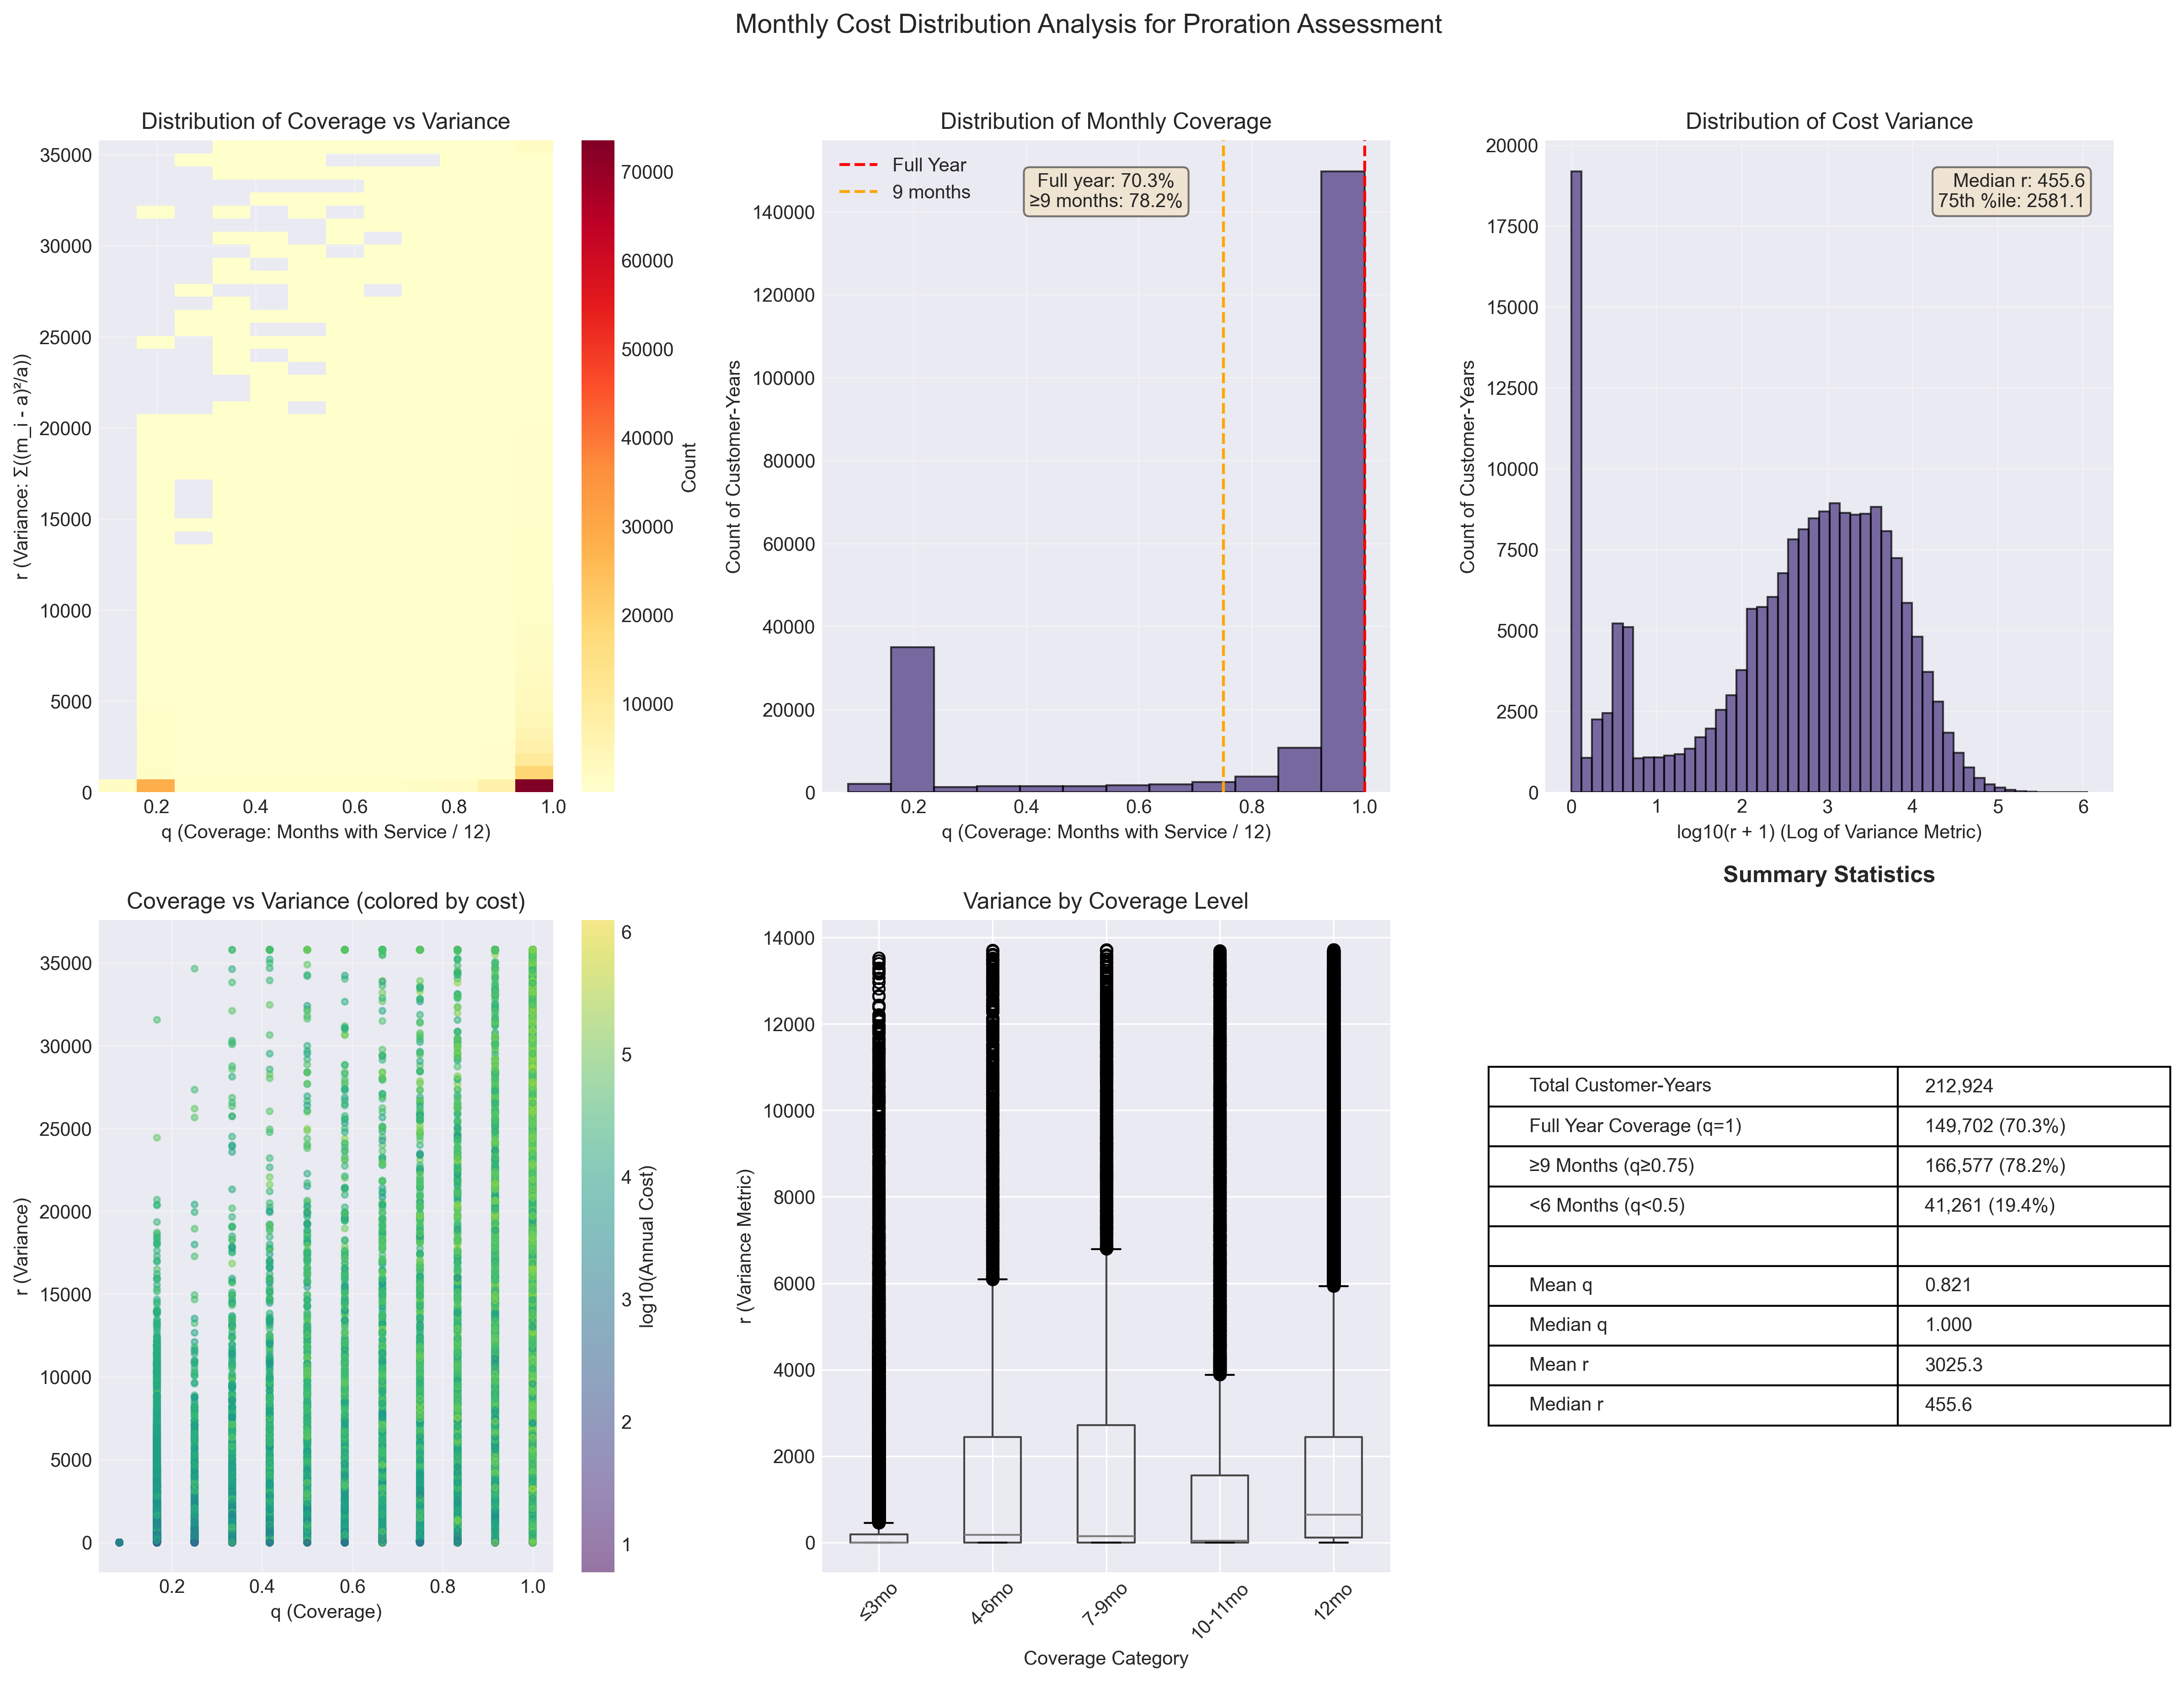
\includegraphics[width=\textwidth]{figures/cost_distribution_analysis.png}
    \caption{Monthly cost distribution analysis for proration assessment}
    \label{fig:proration_analysis}
\end{figure}

Figure~\ref{fig:proration_analysis} presents the comprehensive proration feasibility analysis:

\begin{itemize}
    \item \textbf{Top-left panel}: Two-dimensional histogram showing the relationship between coverage ($q$) and variance ($r$). The concentration of points at $q=1$ demonstrates that most customer-years have complete coverage, while the vertical spread indicates substantial variance in spending patterns.
    
    \item \textbf{Top-center panel}: Distribution of monthly coverage showing a bimodal pattern---customers either have full-year coverage or very limited engagement, with few in between.
    
    \item \textbf{Top-right panel}: Log-scale distribution of the variance metric revealing that cost variance spans multiple orders of magnitude, indicating highly heterogeneous spending patterns.
    
    \item \textbf{Bottom-left panel}: Scatter plot colored by annual cost magnitude shows that higher-cost customers tend to have more complete coverage but also higher variance.
    
    \item \textbf{Bottom-center panel}: Box plots of variance by coverage category reveal the counterintuitive finding that full-year customers have the highest cost variance.
    
    \item \textbf{Bottom-right panel}: Summary statistics quantifying the distribution patterns.
\end{itemize}

The analysis revealed critical findings:
\begin{itemize}
    \item \textbf{\ProrationFullYearPct\% of customer-years} have full 12-month coverage ($q = 1.0$)
    \item \textbf{Median variance for full-year customers}: $r = \ProrationMedianRFull$
    \item \textbf{Median variance for low-coverage customers}: $r = \ProrationMedianRLow$
\end{itemize}

The counterintuitively high variance (\ProrationMedianRFull) for full-year customers indicates highly irregular spending patterns---likely reflecting equipment purchases, hospitalizations, or seasonal service variations. This ``lumpy'' cost distribution makes proration inadvisable for several reasons:

\begin{enumerate}
    \item \textbf{Attribution ambiguity}: With such high monthly variance, costs cannot be fairly attributed to different QSI assessment periods when changes occur mid-year.
    
    \item \textbf{Systematic bias}: The inverse relationship between coverage and variance suggests partial-year customers represent a fundamentally different population that would bias model calibration.
    
    \item \textbf{Implementation complexity}: Any proration scheme would require sophisticated adjustment factors that vary by customer characteristics, introducing additional uncertainty.
\end{enumerate}

Consequently, we maintain the conservative exclusion strategy despite the data loss, as the integrity of the QSI-to-cost relationship is paramount for regulatory compliance and fair budget allocation.

% ⚠ ===================================== ⚠ 

\section{Modeling Framework Architecture}

\subsection{Two-Track Trajectory Modeling}

Given that only \CustomerPctTwoPlusYear\% of customers have sufficient multi-year data for individual trajectory calculation, we implement a dual-track approach:

\subsubsection{Track A: Individual Trajectories}
For the \CustomerNumberTwoPlusYear{} customers with two or more years of usable data:
\begin{enumerate}
    \item Calculate individual linear cost trajectories using ordinary least squares
    \item Store intercept, slope, $R^2$, and years used for each customer
    \item Apply trajectory: $\text{Cost}_{t+k} = \text{Base}_t + k \times \text{Slope}_i$
\end{enumerate}

\subsubsection{Track B: Cluster-Based Trajectories}
For the remaining customers with single-year data:
\begin{enumerate}
    \item Perform K-means clustering on standardized QSI variables and demographics
    \item Assign each customer to their nearest cluster centroid
    \item Inherit the average slope from Track A customers within the same cluster
    \item If cluster contains fewer than 10 Track A customers, use broader grouping
\end{enumerate}

\subsection{Model Calibration Pipeline}

Each of the ten alternative models follows a standardized calibration process:

\begin{enumerate}
    \item \textbf{Feature Preparation}: Apply model-specific transformations and feature engineering
    \item \textbf{Outlier Removal}: Implement model-specific outlier detection (0-10\% removal)
    \item \textbf{Model Fitting}: Train on 80\% of data, stratified by living setting
    \item \textbf{Cross-Validation}: Perform 10-fold stratified cross-validation
    \item \textbf{Trajectory Integration}: Combine base predictions with trajectory adjustments
    \item \textbf{Validation}: Evaluate on 20\% holdout test set
\end{enumerate}

\subsection{Master Pipeline Architecture}

The entire framework operates through a single master script (\texttt{main\_pipeline.py}) that orchestrates all components:

\begin{figure}[h]
\centering
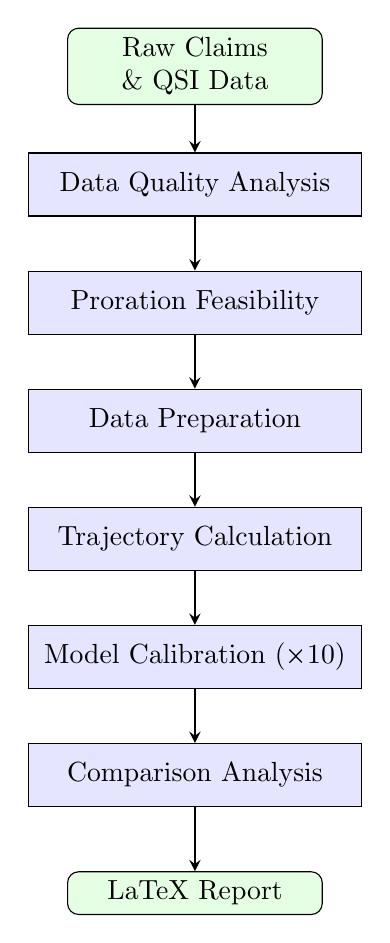
\begin{tikzpicture}[node distance=1.5cm, auto]
    % Define styles
    \tikzstyle{process} = [rectangle, draw, text width=4cm, text centered, minimum height=0.8cm, fill=blue!10]
    \tikzstyle{data} = [rectangle, rounded corners, draw, text width=3cm, text centered, fill=green!10]
    \tikzstyle{arrow} = [thick,->,>=stealth]
    
    % Nodes
    \node [data] (raw) {Raw Claims \& QSI Data};
    \node [process, below of=raw] (quality) {Data Quality Analysis};
    \node [process, below of=quality] (proration) {Proration Feasibility};
    \node [process, below of=proration] (prep) {Data Preparation};
    \node [process, below of=prep] (trajectory) {Trajectory Calculation};
    \node [process, below of=trajectory] (models) {Model Calibration (×10)};
    \node [process, below of=models] (compare) {Comparison Analysis};
    \node [data, below of=compare] (report) {LaTeX Report};
    
    % Arrows
    \draw [arrow] (raw) -- (quality);
    \draw [arrow] (quality) -- (proration);
    \draw [arrow] (proration) -- (prep);
    \draw [arrow] (prep) -- (trajectory);
    \draw [arrow] (trajectory) -- (models);
    \draw [arrow] (models) -- (compare);
    \draw [arrow] (compare) -- (report);
\end{tikzpicture}
\caption{Master pipeline architecture showing sequential processing stages}
\end{figure}

\section{Individual Model Specifications}

\subsection{Model Portfolio}

The framework evaluates ten alternative models, each with distinct theoretical foundations and assumptions:

\begin{enumerate}
    \item \textbf{Current Algorithm Updated}: Square-root transformation with outlier removal
    \item \textbf{GLM-Gamma}: Generalized linear model with gamma distribution and log link
    \item \textbf{Robust Linear Regression}: Huber regression resistant to outliers
    \item \textbf{Weighted Least Squares}: Heteroscedasticity correction through variance weighting
    \item \textbf{Ridge Regression}: L2-regularized regression for multicollinearity
    \item \textbf{Log-Normal}: Linear regression with logarithmic transformation
    \item \textbf{Quantile Regression}: Median-based estimation robust to outliers
    \item \textbf{Bayesian Linear}: Uncertainty quantification through posterior distributions
    \item \textbf{Principal Component Regression}: Dimensionality reduction before regression
    \item \textbf{Deep Learning Network}: Multi-layer neural network for non-linear patterns
\end{enumerate}

\subsection{Common Features}

All models utilize a consistent set of input features:
\begin{itemize}
    \item \textbf{Demographics}: Age groups (0-20, 21-30, 31+)
    \item \textbf{Living Settings}: Family home, independent/supported living, residential homes (1-4)
    \item \textbf{QSI Variables}: Q16, Q18, Q20, Q21, Q23, Q28, Q33, Q34, Q36, Q43
    \item \textbf{Sum Scores}: BSum, FHFSum, SLFSum, SLBSum
    \item \textbf{Temporal}: Fiscal year as numeric feature
\end{itemize}

\section{Validation Strategy}

\subsection{Dual Validation Approach}

Models undergo two complementary validation strategies:

\subsubsection{Temporal Validation}
\begin{itemize}
    \item Training: Fiscal years 2018-2022
    \item Testing: Fiscal years 2023-2024
    \item Metrics: Year-ahead prediction accuracy
\end{itemize}

\subsubsection{Cross-Sectional Validation}
\begin{itemize}
    \item 80/20 train-test split stratified by living setting
    \item 10-fold cross-validation on training set
    \item Bootstrap confidence intervals (100 iterations)
\end{itemize}

\subsection{Performance Metrics}

Each model is evaluated using comprehensive metrics:
\begin{itemize}
    \item \textbf{Regression accuracy}: $R^2$, adjusted $R^2$, RMSE, MAE, MAPE
    \item \textbf{Model selection}: AIC, BIC
    \item \textbf{Robustness}: Performance by demographic subgroups
    \item \textbf{Trajectory accuracy}: Multi-year prediction errors
    \item \textbf{Fairness}: Disparate impact analysis across protected classes
\end{itemize}

\section{Reproducibility and Quality Assurance}

\subsection{Configuration Management}

All parameters are externalized in JSON configuration files:
\begin{itemize}
    \item \texttt{master\_config.json}: Global settings, paths, and thresholds
    \item \texttt{model\_configs/}: Individual model hyperparameters
    \item Version control through Git ensures configuration tracking
\end{itemize}

\subsection{Reproducibility Features}

\begin{enumerate}
    \item \textbf{Random seed control}: Fixed seed (42) for all stochastic operations
    \item \textbf{Checkpoint system}: Intermediate results saved for debugging/restart
    \item \textbf{Comprehensive logging}: Detailed logs at each pipeline stage
    \item \textbf{Data versioning}: MD5 checksums for input data files
    \item \textbf{Environment specification}: Docker container for consistent execution
\end{enumerate}

\subsection{Quality Checks}

Automated quality checks ensure data and model integrity:
\begin{itemize}
    \item Verification that excluded records match documented criteria
    \item Comparison of model coefficients against expected ranges
    \item Detection of data leakage between train and test sets
    \item Validation of LaTeX output compilation
    \item Performance regression tests against baseline metrics
\end{itemize}

\section{Technical Architecture and Implementation Framework}

\subsection{System Architecture Overview}

The iBudget model calibration framework implements a hierarchical object-oriented architecture designed for extensibility, reproducibility, and maintainability. The system employs the Template Method design pattern, where a base abstract class defines the algorithmic skeleton while allowing derived classes to override specific steps.

\subsection{Class Hierarchy and Design Patterns}

\subsubsection{Base Abstract Class}

The \texttt{BaseISFModel} abstract class serves as the foundation for all ten alternative models. It enforces a consistent interface while allowing model-specific implementations:

\begin{verbatim}
class BaseISFModel(ABC):
    def __init__(self, model_id: int, model_name: str, config: Dict)
    
    @abstractmethod
    def prepare_features(self, data: pd.DataFrame) -> pd.DataFrame
    
    @abstractmethod
    def build_model(self) -> None
    
    @abstractmethod
    def get_model_specific_params(self) -> Dict[str, Any]
    
    # Concrete methods shared across all models
    def fit(self, X_train, y_train) -> 'BaseISFModel'
    def predict(self, X: pd.DataFrame) -> np.ndarray
    def evaluate(self, X_test, y_test) -> Dict[str, float]
    def cross_validate(self, X, y, cv=10) -> Dict[str, Any]
    def generate_diagnostic_plots(self, X_test, y_test) -> None
    def to_tex(self, output_path: Optional[Path]) -> Path
    def save_metrics(self) -> None
\end{verbatim}

\subsubsection{Derived Model Classes}

Each alternative model extends \texttt{BaseISFModel} with specific implementations:

\begin{itemize}
    \item \textbf{Alternative1Model}: Implements square-root transformation with percentile-based outlier removal
    \item \textbf{Alternative2Model}: GLM with Gamma family using statsmodels or sklearn's TweedieRegressor
    \item \textbf{Alternative3Model}: HuberRegressor for robust regression
    \item \textbf{Alternative4Model}: Weighted Least Squares with heteroscedasticity correction
    \item \textbf{Alternative5Model}: RidgeCV with cross-validated alpha selection
    \item \textbf{Alternative6Model}: Log-normal regression with smearing adjustment
    \item \textbf{Alternative7Model}: Quantile regression for median estimation
    \item \textbf{Alternative8Model}: BayesianRidge for uncertainty quantification
    \item \textbf{Alternative9Model}: PCA-based dimensionality reduction pipeline
    \item \textbf{Alternative10Model}: Neural network using Keras/TensorFlow or MLPRegressor
\end{itemize}

\subsection{Directory Structure}

The project follows a modular directory structure that separates code, configuration, data, and outputs:

\begin{verbatim}
iBudget/
├── script/                          # All Python code
│   ├── main_pipeline.py            # Master orchestration script
│   ├── data_quality/
│   │   ├── outlier_analysis.py     # Outlier detection and statistics
│   │   └── proration_analysis.py   # Monthly cost distribution analysis
│   ├── models/
│   │   ├── __init__.py
│   │   ├── base_model.py           # Abstract base class
│   │   ├── alternative_1.py        # Current algorithm updated
│   │   ├── alternative_2.py        # GLM Gamma
│   │   ├── alternative_3.py        # Robust regression
│   │   ├── alternative_4.py        # Weighted least squares
│   │   ├── alternative_5.py        # Ridge regression
│   │   ├── alternative_6.py        # Log-normal
│   │   ├── alternative_7.py        # Quantile regression
│   │   ├── alternative_8.py        # Bayesian linear
│   │   ├── alternative_9.py        # Principal component regression
│   │   └── alternative_10.py       # Deep learning network
│   ├── trajectory/
│   │   ├── calculator.py           # Individual trajectory calculation
│   │   └── clustering.py           # QSI-based clustering for imputation
│   ├── utils/
│   │   ├── database.py             # Database connection utilities
│   │   ├── metrics.py              # Performance metric calculations
│   │   └── visualization.py        # Common plotting functions
│   └── configs/
│       ├── master_config.json      # Global configuration
│       └── model_configs/          # Individual model parameters
│           ├── model_1_config.json
│           └── ...
├── report/                          # LaTeX and output files
│   ├── iBudget.tex                 # Main document
│   ├── 0.1.config.tex              # Document configuration
│   ├── Methodology.tex             # This methodology chapter
│   ├── data_quality_commands.tex   # Dynamic statistics
│   ├── proration_commands.tex      # Proration statistics
│   ├── figures/                    # All generated plots
│   ├── models/                     # Model-specific outputs
│   │   ├── alternative_1/
│   │   │   ├── Alternative_1_calibrated.tex
│   │   │   ├── plots/
│   │   │   └── metrics.json
│   │   └── ...
│   └── comparison/                 # Cross-model comparisons
│       ├── model_comparison_master.tex
│       └── comparative_plots/
├── data/                            # Data storage
│   ├── raw/                        # Original data files
│   ├── processed/                  # Cleaned datasets
│   └── intermediate/               # Checkpoint saves
└── logs/                            # Execution logs
    └── pipeline_YYYYMMDD_HHMMSS.log
\end{verbatim}

\subsection{Configuration Management}

\subsubsection{Master Configuration Structure}

The \texttt{master\_config.json} provides centralized control over all pipeline parameters:

\begin{verbatim}
{
  "master_config": {
    "project_name": "Florida iBudget Algorithm Calibration",
    "version": "1.0.0",
    "data_settings": {
      "database": "APD",
      "server": ".",
      "random_seed": 42,
      "test_size": 0.2,
      "cv_folds": 10
    },
    "common_features": {
      "demographic": ["age_group", "living_setting"],
      "qsi_variables": ["Q16", "Q18", "Q20", "Q21", "Q23", 
                        "Q28", "Q33", "Q34", "Q36", "Q43"],
      "sum_scores": ["BSum", "FHFSum", "SLFSum", "SLBSum"]
    },
    "output_settings": {
      "report_dir": "../report",
      "models_dir": "../report/models",
      "figures_dir": "../report/figures",
      "log_dir": "../logs"
    }
  }
}
\end{verbatim}

\subsubsection{Model-Specific Configurations}

Each model maintains its own configuration file with hyperparameters:

\begin{verbatim}
{
  "model_id": 1,
  "model_name": "Current Algorithm Updated",
  "transformation": "sqrt",
  "outlier_removal": {
    "method": "percentile",
    "threshold": 0.094
  },
  "features": {
    "use_common": true,
    "additional": [],
    "exclude": []
  }
}
\end{verbatim}

\subsection{Data Flow and Processing Pipeline}

\subsubsection{Pipeline Execution Sequence}

The master pipeline orchestrates execution through defined stages:

\begin{enumerate}
    \item \textbf{Initialization}: Load configurations, establish database connections
    \item \textbf{Data Quality Analysis}: Execute \texttt{sp\_Outliers}, generate exclusion statistics
    \item \textbf{Proration Analysis}: Analyze monthly distributions, document decision
    \item \textbf{Data Preparation}: Apply exclusions, create customer-fiscal year dataset
    \item \textbf{Feature Engineering}: Prepare common and model-specific features
    \item \textbf{Trajectory Calculation}: Compute individual slopes, perform clustering
    \item \textbf{Model Calibration}: Sequential or parallel model fitting
    \item \textbf{Validation}: Cross-validation and holdout testing
    \item \textbf{Comparison}: Generate comparative metrics and visualizations
    \item \textbf{Report Generation}: Compile LaTeX outputs
\end{enumerate}

\subsubsection{Checkpoint and Recovery System}

The pipeline implements checkpointing for fault tolerance:

\begin{verbatim}
checkpoint_manager = CheckpointManager(checkpoint_dir='../data/intermediate')

# Save checkpoint after each major stage
checkpoint_manager.save('data_prepared', {
    'X_train': X_train,
    'X_test': X_test,
    'y_train': y_train,
    'y_test': y_test
})

# Recovery on restart
if checkpoint_manager.exists('data_prepared'):
    data = checkpoint_manager.load('data_prepared')
    X_train = data['X_train']
    # ... continue from checkpoint
\end{verbatim}

\subsection{Key Implementation Classes}

\subsubsection{ModelPipeline Class}

The central orchestrator managing the entire workflow:

\begin{verbatim}
class ModelPipeline:
    def __init__(self, config_path: str)
    def load_data(self) -> pd.DataFrame
    def validate_data(self) -> None
    def prepare_common_features(self) -> pd.DataFrame
    def split_data(self, features, target) -> None
    def calibrate_single_model(self, model_config) -> BaseISFModel
    def calibrate_all_models(self) -> None
    def generate_comparisons(self) -> None
    def run(self) -> None
\end{verbatim}

\subsubsection{TrajectoryCalculator Class}

Handles the two-track trajectory modeling:

\begin{verbatim}
class TrajectoryCalculator:
    def calculate_individual_slopes(self, customer_data) -> Dict
    def perform_qsi_clustering(self, n_clusters=30) -> KMeans
    def assign_cluster_slopes(self, customers_without_trajectory) -> Dict
    def get_trajectory_adjustment(self, customer_id, years_forward) -> float
\end{verbatim}

\subsubsection{ModelComparison Class}

Generates cross-model analytics:

\begin{verbatim}
class ModelComparison:
    def __init__(self, models: List[BaseISFModel])
    def generate_comparison_matrix(self) -> pd.DataFrame
    def generate_performance_summary(self) -> None
    def calculate_prediction_correlation(self) -> pd.DataFrame
    def generate_master_tex(self) -> Path
\end{verbatim}

\subsection{Database Integration}

\subsubsection{Connection Management}

Database connections use Windows Authentication with connection pooling:

\begin{verbatim}
class DatabaseManager:
    def __init__(self):
        self.connection_string = (
            "DRIVER={ODBC Driver 17 for SQL Server};"
            "SERVER=.;DATABASE=APD;Trusted_Connection=yes"
        )
        self.connection_pool = []
    
    def get_connection(self) -> pyodbc.Connection
    def execute_query(self, query: str) -> pd.DataFrame
    def execute_stored_procedure(self, sp_name: str) -> List[pd.DataFrame]
\end{verbatim}

\subsubsection{Key Database Objects}

The system interacts with these primary database objects:

\begin{itemize}
    \item \textbf{tbl\_Claims\_MMIS}: Service claims with dates and paid amounts
    \item \textbf{tbl\_QSIAssessments}: QSI scores and assessment dates
    \item \textbf{sp\_Outliers}: Analyzes data quality and exclusions
    \item \textbf{sp\_PrepareModelingData}: Creates customer-fiscal year dataset
\end{itemize}

\subsection{Quality Assurance and Testing}

\subsubsection{Unit Testing Framework}

Each model class includes comprehensive unit tests:

\begin{verbatim}
class TestAlternative1Model(unittest.TestCase):
    def setUp(self):
        self.model = Alternative1Model(model_id=1, ...)
        self.test_data = generate_test_data()
    
    def test_feature_preparation(self):
        features = self.model.prepare_features(self.test_data)
        self.assertEqual(features.shape[1], 21)
    
    def test_outlier_removal(self):
        # Verify correct percentage removed
    
    def test_model_convergence(self):
        # Ensure model fits without errors
\end{verbatim}

\subsubsection{Integration Testing}

End-to-end pipeline tests verify complete workflow:

\begin{itemize}
    \item Data loading and validation
    \item Feature engineering consistency
    \item Model calibration completion
    \item LaTeX compilation success
    \item Performance regression checks
\end{itemize}

\subsection{Performance Optimization}

\subsubsection{Parallel Processing}

Independent models are calibrated in parallel using multiprocessing:

\begin{verbatim}
from multiprocessing import Pool

def calibrate_models_parallel(model_configs):
    with Pool(processes=4) as pool:
        models = pool.map(calibrate_single_model, model_configs)
    return models
\end{verbatim}

\subsubsection{Memory Management}

Large datasets are processed in chunks to manage memory:

\begin{verbatim}
def process_in_chunks(data, chunk_size=10000):
    for start in range(0, len(data), chunk_size):
        chunk = data[start:start + chunk_size]
        yield process_chunk(chunk)
\end{verbatim}

\subsection{Logging and Monitoring}

\subsubsection{Hierarchical Logging}

Multi-level logging captures execution details:

\begin{verbatim}
logging.config.dictConfig({
    'version': 1,
    'handlers': {
        'file': {
            'class': 'logging.FileHandler',
            'filename': f'pipeline_{timestamp}.log',
            'level': 'DEBUG'
        },
        'console': {
            'class': 'logging.StreamHandler',
            'level': 'INFO'
        }
    },
    'root': {
        'handlers': ['file', 'console']
    }
})
\end{verbatim}

\subsubsection{Performance Metrics}

Execution timing and resource usage are tracked:

\begin{verbatim}
@timing_decorator
def calibrate_model(model_config):
    start_memory = get_memory_usage()
    # ... model calibration
    end_memory = get_memory_usage()
    log_performance_metrics(time_elapsed, memory_used)
\end{verbatim}

\subsection{Deployment Considerations}

\subsubsection{Environment Setup}

Required Python packages and versions:

\begin{verbatim}
# requirements.txt
pandas>=1.3.0
numpy>=1.21.0
scikit-learn>=1.0.0
statsmodels>=0.13.0
tensorflow>=2.8.0  # For Alternative 10
pyodbc>=4.0.0
matplotlib>=3.4.0
seaborn>=0.11.0
\end{verbatim}

\subsubsection{Docker Containerization}

For reproducible environments:

\begin{verbatim}
FROM python:3.9
WORKDIR /app
COPY requirements.txt .
RUN pip install -r requirements.txt
COPY script/ ./script/
CMD ["python", "script/main_pipeline.py"]
\end{verbatim}

\subsection{Summary}

This technical architecture provides a robust, scalable framework for the iBudget model calibration project. The object-oriented design ensures code reusability and maintainability, while the modular structure facilitates independent development and testing of components. The comprehensive configuration management and checkpoint system ensure reproducibility and fault tolerance, critical for regulatory compliance and scientific validity.

\subsection{Computational Requirements}

\begin{itemize}
    \item \textbf{Hardware}: Minimum 16GB RAM, 8 CPU cores recommended
    \item \textbf{Execution time}: Complete pipeline $<$2 hours, individual model $<$10 minutes
    \item \textbf{Storage}: Approximately 5GB for intermediate files and outputs
    \item \textbf{Parallelization}: Independent models processed concurrently when possible
\end{itemize}

\subsection{Risk Mitigation}

Key risks and mitigation strategies:
\begin{enumerate}
    \item \textbf{Limited trajectory coverage}: Clustering approach ensures all consumers receive trajectory adjustments
    \item \textbf{High cost variance}: Multiple outlier detection methods to identify appropriate thresholds
    \item \textbf{Model overfitting}: Cross-validation and regularization prevent overspecialization
    \item \textbf{Technical failures}: Checkpoint system enables pipeline restart without data loss
\end{enumerate}

\section{Summary}

This methodology provides a comprehensive framework for evaluating alternative iBudget algorithms while addressing significant data quality challenges. The conservative exclusion strategy, justified by the proration analysis, ensures model calibration uses only high-quality data. The two-track trajectory approach accommodates limited longitudinal coverage, while the unified pipeline architecture ensures reproducibility and comparability across all models. This systematic approach enables evidence-based selection of the optimal algorithm for Florida's disability services allocation.